\documentclass[12pt,a4paper]{report}
\usepackage{fontspec}
\usepackage{amsmath,amssymb,amsthm}
\usepackage{array,booktabs,longtable,multirow}
\usepackage[margin=2.3cm,headheight=15pt]{geometry}
\usepackage{enumitem}
\usepackage[table]{xcolor}
\usepackage{titlesec}
\usepackage{mdframed}
\usepackage{fancyhdr}
\usepackage{graphicx}
\usepackage{float}
\usepackage{listings}
\usepackage[hidelinks]{hyperref}

\setmainfont{Times New Roman}
\setsansfont{Arial}[Scale=0.92]
\setmonofont{Courier New}[Scale=0.92]

\definecolor{dnavy}{HTML}{123A6B}
\definecolor{dred}{HTML}{B02418}
\definecolor{dgray}{HTML}{F2F4F7}

\titleformat{\chapter}[hang]{\sffamily\LARGE\bfseries\color{dnavy}}{Chương \thechapter.}{0.6em}{}
\titlespacing*{\chapter}{0pt}{0pt}{14pt}
\titleformat{\section}{\sffamily\large\bfseries\color{dnavy}}{\thesection}{0.6em}{}
\titleformat{\subsection}{\sffamily\normalsize\bfseries\color{dred}}{\thesubsection}{0.6em}{}
\renewcommand{\contentsname}{Mục lục}
\renewcommand{\figurename}{Hình}
\renewcommand{\tablename}{Bảng}
\renewcommand{\bibname}{Tài liệu tham khảo}
\renewcommand{\appendixname}{Phụ lục}

\newmdenv[backgroundcolor=dgray,linewidth=0pt,skipabove=6pt,skipbelow=6pt,innertopmargin=6pt,innerbottommargin=6pt]{note}
\setlist[enumerate]{itemsep=2pt,topsep=3pt}
\setlist[itemize]{itemsep=2pt,topsep=3pt}
\lstset{basicstyle=\ttfamily\small,columns=fullflexible,keepspaces=true,frame=single,
  rulecolor=\color{black!20},backgroundcolor=\color{dgray},numbers=left,numberstyle=\tiny\color{gray},
  xleftmargin=1.5em,breaklines=true,showstringspaces=false}

\pagestyle{fancy}\fancyhf{}
\lhead{\small\sffamily CS112 -- Phân tích \& Thiết kế thuật toán}
\rhead{\small\sffamily Bài tập lớn -- Đường đi an toàn}
\cfoot{\small\thepage}
\renewcommand{\headrulewidth}{0.4pt}
\fancypagestyle{plain}{\fancyhf{}\cfoot{\small\thepage}\renewcommand{\headrulewidth}{0pt}}

\newcommand{\ExMap}{\begin{tabular}{c|cccccc}
 & 1 & 2 & 3 & 4 & 5 & 6\\\hline
1 & KTX & . & . & . & . & .\\
2 & . & \textbf{*} & . & . & . & .\\
3 & . & . & . & \textbf{*} & . & .\\
4 & \textbf{*} & . & . & . & . & .\\
5 & . & . & \textbf{*} & . & . & .\\
6 & . & . & . & . & . & UIT\\
\end{tabular}}
\newcommand{\ExTable}{\begin{tabular}{c|cccccc}
$dp$ & 1 & 2 & 3 & 4 & 5 & 6\\\hline
1 & 1 & 1 & 1 & 1 & 1 & 1\\
2 & 1 & \cellcolor{red!12}0 & 1 & 2 & 3 & 4\\
3 & 1 & 1 & 2 & \cellcolor{red!12}0 & 3 & 7\\
4 & \cellcolor{red!12}0 & 1 & 3 & 3 & 6 & 13\\
5 & 0 & 1 & \cellcolor{red!12}0 & 3 & 9 & 22\\
6 & 0 & 1 & 1 & 4 & 13 & \cellcolor{yellow!35}\textbf{35}\\
\end{tabular}}
\newcommand{\ExRows}{\begin{longtable}{>{\centering\arraybackslash}p{0.8cm} >{\raggedright\arraybackslash}p{9.2cm} >{\centering\arraybackslash}p{4.3cm}}
\toprule
Hàng & Các thao tác trên mảng $dp[1..6]$ & $dp$ sau hàng\\\midrule\endhead
-- & Khởi tạo & $[1,0,0,0,0,0]$\\\midrule
1 & $dp[1]=1$ (KTX); $dp[2]\leftarrow 0+1=1$; $dp[3]\leftarrow 0+1=1$; $dp[4]\leftarrow 0+1=1$; $dp[5]\leftarrow 0+1=1$; $dp[6]\leftarrow 0+1=1$ & $[1,1,1,1,1,1]$\\\midrule
2 & $dp[1]$ giữ 1; $dp[2]\leftarrow 0$ (chốt); $dp[3]\leftarrow 1+0=1$; $dp[4]\leftarrow 1+1=2$; $dp[5]\leftarrow 1+2=3$; $dp[6]\leftarrow 1+3=4$ & $[1,0,1,2,3,4]$\\\midrule
3 & $dp[1]$ giữ 1; $dp[2]\leftarrow 0+1=1$; $dp[3]\leftarrow 1+1=2$; $dp[4]\leftarrow 0$ (chốt); $dp[5]\leftarrow 3+0=3$; $dp[6]\leftarrow 4+3=7$ & $[1,1,2,0,3,7]$\\\midrule
4 & $dp[1]\leftarrow 0$ (chốt); $dp[2]\leftarrow 1+0=1$; $dp[3]\leftarrow 2+1=3$; $dp[4]\leftarrow 0+3=3$; $dp[5]\leftarrow 3+3=6$; $dp[6]\leftarrow 7+6=13$ & $[0,1,3,3,6,13]$\\\midrule
5 & $dp[1]$ giữ 0; $dp[2]\leftarrow 1+0=1$; $dp[3]\leftarrow 0$ (chốt); $dp[4]\leftarrow 3+0=3$; $dp[5]\leftarrow 6+3=9$; $dp[6]\leftarrow 13+9=22$ & $[0,1,0,3,9,22]$\\\midrule
6 & $dp[1]$ giữ 0; $dp[2]\leftarrow 1+0=1$; $dp[3]\leftarrow 0+1=1$; $dp[4]\leftarrow 3+1=4$; $dp[5]\leftarrow 9+4=13$; $dp[6]\leftarrow 22+13=35$ & $[0,1,1,4,13,35]$\\\midrule
\bottomrule\end{longtable}}
\newcommand{\ExIE}{\begin{longtable}{c c >{\raggedright\arraybackslash}p{9.6cm} c}
\toprule
Bước & Điểm & Công thức & $g$\\\midrule\endhead
1 & \#1\,(2,2) & $\binom{2}{1} = 2$ & 2\\
2 & \#2\,(3,4) & $\binom{5}{2} - g_{1}\cdot\binom{3}{1} = 10 - 2\cdot 3$ & 4\\
3 & \#3\,(4,1) & $\binom{3}{3} = 1$ & 1\\
4 & \#4\,(5,3) & $\binom{6}{4} - g_{1}\cdot\binom{4}{3} - g_{3}\cdot\binom{3}{1} = 15 - 2\cdot 4 - 1\cdot 3$ & 4\\
5 & UIT (6,6) & $\binom{10}{5} - g_{1}\cdot\binom{8}{4} - g_{2}\cdot\binom{5}{3} - g_{3}\cdot\binom{7}{2} - g_{4}\cdot\binom{4}{1} = 252 - 2\cdot 70 - 4\cdot 10 - 1\cdot 21 - 4\cdot 4$ & \textbf{35}\\
\bottomrule\end{longtable}}
\newcommand{\ExOpsBrute}{146}\newcommand{\ExOpsMemo}{63}\newcommand{\ExOpsDp}{36}\newcommand{\ExOpsIe}{22}\newcommand{\ExHits}{13}\newcommand{\ExCalls}{63}\newcommand{\ExDepth}{11}

\newcommand{\demo}{\url{https://vanhuydotcom.github.io/cs112-duong-di-an-toan/}}

\begin{document}

% ==================== TRANG BÌA ====================
\begin{titlepage}
\centering
\vspace*{0.4cm}
{\large ĐẠI HỌC QUỐC GIA THÀNH PHỐ HỒ CHÍ MINH}\\[4pt]
{\large\bfseries TRƯỜNG ĐẠI HỌC CÔNG NGHỆ THÔNG TIN}\\[4pt]
{\large KHOA KHOA HỌC MÁY TÍNH}\\[1.2cm]
\rule{\linewidth}{1pt}\\[10pt]
{\Large\bfseries\color{dnavy} BÁO CÁO BÀI TẬP LỚN}\\[14pt]
{\LARGE\bfseries ĐƯỜNG ĐI AN TOÀN}\\[10pt]
{\large\itshape Demo trực quan hóa và so sánh bốn cách giải\\bài toán đếm đường đi trên lưới có vật cản}\\[10pt]
\rule{\linewidth}{1pt}\\[1.4cm]
\begin{tabular}{@{}>{\bfseries}l l@{}}
Môn học: & Phân tích \& Thiết kế thuật toán (CS112) \\[6pt]
Lớp: & CS112.2026.TX \\[6pt]
Giảng viên: & Huỳnh Thị Thanh Thương \\[6pt]
Sinh viên: & Đinh Văn Huy -- 25730032 \\[6pt]
Hình thức: & Cá nhân \\[6pt]
Demo online: & \demo \\[6pt]
Mã nguồn: & \url{https://github.com/vanhuydotcom/cs112-duong-di-an-toan}\\
\end{tabular}
\vfill
{\large TP. Hồ Chí Minh, tháng 10 năm 2026}
\end{titlepage}

\tableofcontents

% =====================================================
\chapter{Giới thiệu bài toán}
\section{Lý do chọn bài toán}
Em chọn bài \textbf{``Đường đi an toàn''} vì đây là bài em \textbf{đã tự giải và nộp đạt (Accepted) trong assignment Quy hoạch động trên WeCode} của lớp. Vì đã nắm chắc lời giải, em muốn phát triển nó thành một demo để \emph{nhìn thấy} quy hoạch động hoạt động ra sao, thay vì chỉ có một đoạn code được chấm đúng. Bài toán cũng có ưu điểm là rất dễ hình dung: mỗi ô của bảng quy hoạch động chính là một ô trên bản đồ, nên việc ``điền bảng'' có thể diễn ra trực tiếp trên bản đồ.

Khi cô cập nhật yêu cầu (khuyến khích giải bằng nhiều cách rồi so sánh), em mở rộng demo thành \textbf{bốn cách giải}: vét cạn quay lui, đệ quy có nhớ, quy hoạch động bottom-up và tổ hợp kết hợp bao hàm--loại trừ. Bốn cách này nối các chủ đề của môn (quay lui, quy hoạch động, kỹ thuật đếm sơ cấp ở Buổi 1) vào cùng một bài toán.

\section{Nguồn gốc}
\begin{itemize}
  \item Đề bài lấy từ WeCode, assignment Quy hoạch động của lớp CS112.2026.TX (câu chuyện ``Tấn Lưu'' đi từ KTX khu B tới UIT).
  \item Đây là một dạng kinh điển của bài toán \emph{đếm đường đi trên lưới} (lattice paths). Bài ``Grid Paths'' trong CSES Problem Set~\cite{cses} có cùng phát biểu và cùng giới hạn ($n \le 1000$, lấy dư $10^9+7$).
  \item Kỹ thuật tổ hợp + bao hàm--loại trừ trên các ô bị cấm là kỹ thuật đã biết, xuất hiện trong bài ``Gerald and Giant Chess'' (Codeforces 559C)~\cite{cf559c}. Em tham khảo ý tưởng này qua gợi ý của AI và trình bày lại, chứng minh lại ở Chương~4.
\end{itemize}

\section{Ứng dụng thực tế}
\begin{itemize}
  \item \textbf{Định tuyến trên lưới đường phố} (kiểu Manhattan): đếm số tuyến đường ngắn nhất giữa hai giao lộ khi có đoạn đường bị cấm, sửa chữa hoặc tắc nghẽn.
  \item \textbf{Robot trong nhà kho} hoặc bản đồ ô vuông: đếm, liệt kê các lộ trình đơn điệu tránh vật cản, làm cơ sở để chọn lộ trình ít rủi ro.
  \item \textbf{Xác suất}: số đường an toàn chia cho tổng số đường cho ra xác suất một lộ trình ngẫu nhiên tránh được mọi chốt.
  \item \textbf{Nền tảng của nhiều bài QHĐ trên lưới}: LCS, khoảng cách chỉnh sửa (edit distance), dóng hàng chuỗi trong sinh học đều là QHĐ trên đồ thị có hướng không chu trình dạng lưới. Mỗi ô phụ thuộc ô trên, ô trái (và ô chéo), giống hệt bài này.
\end{itemize}

% =====================================================
\chapter{Mô tả bài toán}
\begin{note}
\textbf{ĐƯỜNG ĐI AN TOÀN.} Tấn Lưu muốn chở bạn từ ký túc xá khu B về trường UIT nhưng sợ bị cảnh sát giao thông thổi. Anh có bản đồ làng đại học kích thước $n\times n$; một số ô có chốt CSGT. KTX khu B ở ô $[1,1]$ (góc trái trên), UIT ở ô $[n,n]$ (góc phải dưới). Mỗi bước Tấn Lưu chỉ được đi \textbf{sang phải} hoặc \textbf{xuống dưới}. Một con đường là \emph{an toàn} nếu không đi qua ô nào có chốt. Hãy đếm số con đường an toàn.

\textbf{Input.} Dòng đầu là số nguyên dương $n$ ($1\le n\le 1000$). $n$ dòng tiếp theo, mỗi dòng gồm $n$ ký tự: `\texttt{.}' là ô trống, `\texttt{*}' là ô có chốt.

\textbf{Output.} Một số nguyên duy nhất: số đường đi an toàn, lấy dư cho $10^9+7$.
\end{note}

\begin{center}
\begin{tabular}{p{4.0cm} p{2.4cm} p{7.4cm}}
\toprule
\textbf{Input} & \textbf{Output} & \textbf{Giải thích}\\\midrule
\texttt{4}\newline\texttt{....}\newline\texttt{.*..}\newline\texttt{...*}\newline\texttt{*...} & \texttt{3} & Ví dụ trong đề (hình minh họa trên WeCode).\\\midrule
\texttt{1}\newline\texttt{*} & \texttt{0} & Chốt ngay tại KTX: không có đường nào.\\\midrule
\texttt{20}, không có chốt & \texttt{345263555} & $\binom{38}{19}=35\,345\,263\,800 > 10^9+7$, phải lấy dư.\\
\bottomrule
\end{tabular}
\end{center}

% =====================================================
\chapter{Mô hình bài toán}
\section{Input}
\begin{itemize}
  \item $n \in \mathbb{Z}$, $1\le n\le 1000$: kích thước bản đồ.
  \item $A=(a_{ij})_{n\times n}$, $a_{ij}\in\{\texttt{.},\texttt{*}\}$: bản đồ, $a_{ij}=\texttt{*}$ khi ô $(i,j)$ có chốt.
\end{itemize}
\section{Output}
$R = |\mathcal{P}| \bmod (10^9+7)$, với $0\le R<10^9+7$. Ở đây $\mathcal{P}$ là tập các dãy ô $c_0=(1,1),c_1,\dots,c_{2n-2}=(n,n)$ thỏa:
(i) $c_{t+1}$ bằng $c_t+(0,1)$ hoặc $c_t+(1,0)$; (ii) $a_{c_t}=\texttt{.}$ với mọi $t$.
\section{Ràng buộc và nhận xét}
\begin{itemize}
  \item Mọi đường đều có đúng $2n-2$ bước ($n-1$ bước xuống, $n-1$ bước phải), nên tổng số đường không có chốt là $\binom{2n-2}{n-1}$. Với $n=1000$ con số này có $\approx 600$ chữ số, vì thế đề yêu cầu lấy dư.
  \item Nếu $(1,1)$ hoặc $(n,n)$ có chốt thì $R=0$.
  \item Input có thể sai định dạng (khi người dùng nhập tay trên demo): $n$ không phải số nguyên, $n$ ngoài $[1,1000]$, thiếu hoặc thừa dòng, dòng sai độ dài, ký tự lạ. Demo kiểm tra đủ các trường hợp này (Chương~7, nhóm 6).
\end{itemize}

% =====================================================
\chapter{Thiết kế cấu trúc dữ liệu và thuật toán}
\section{Phân tích đặc trưng của bài toán}
\begin{enumerate}
  \item \textbf{Đồ thị có hướng không chu trình (DAG).} Coi mỗi ô trống là một đỉnh, có cung $(i,j)\to(i,j+1)$ và $(i,j)\to(i+1,j)$. Do chỉ đi phải/xuống nên không có chu trình. Bài toán trở thành \emph{đếm số đường đi từ nguồn tới đích trong DAG}.
  \item \textbf{Bài toán con gối nhau.} Số đường tới ô $(i,j)$ chỉ phụ thuộc vào ô đó, không phụ thuộc đường đi tiếp theo. Rất nhiều đường dùng chung đoạn đầu, nên liệt kê từng đường (vét cạn) sẽ tính lặp lại khối lượng khổng lồ.
  \item \textbf{Phân hoạch theo bước cuối.} Mọi đường tới $(i,j)$ có bước cuối từ trên hoặc từ trái; hai nhóm rời nhau, cho ra công thức truy hồi cộng.
  \item \textbf{Cấu trúc tổ hợp.} Khi không có chốt, số đường giữa hai ô có công thức đóng $\binom{\Delta i+\Delta j}{\Delta i}$. Nếu số chốt $k$ nhỏ, ta có thể chỉ làm việc trên $k$ chốt thay vì $n^2$ ô.
\end{enumerate}

\section{Cấu trúc dữ liệu}
\begin{center}
\begin{tabular}{p{4.3cm} p{5.6cm} p{4.6cm}}
\toprule
\textbf{Thành phần} & \textbf{Tổ chức} & \textbf{Dùng ở}\\\midrule
Bản đồ & Ma trận $n\times n$ giá trị logic (\texttt{true} = chốt) & Mọi cách giải\\
Bảng $dp$ 1 chiều & Mảng $n$ số nguyên (mod $p$) & QHĐ bottom-up (lời giải nộp)\\
Bảng $dp$ 2 chiều & Ma trận $n\times n$ số nguyên lớn (BigInt) & Demo: hiển thị số thật trước khi lấy dư\\
Bảng nhớ \texttt{memo} & Mảng $n^2$ số nguyên, $-1$ = chưa tính & Đệ quy có nhớ\\
Ngăn xếp tường minh & Mảng các khung $(i,j,\text{giai đoạn})$ & Đệ quy có nhớ, vét cạn (tránh tràn stack)\\
Danh sách chốt & Mảng các cặp $(i,j)$ sắp theo (hàng, cột) & Bao hàm--loại trừ\\
Giai thừa, nghịch đảo & Hai mảng $2n+1$ phần tử mod $p$ & Tính $\binom{a}{b}$ trong $O(1)$\\
\bottomrule
\end{tabular}
\end{center}
Trong cài đặt JavaScript, phép nhân hai số $<p\approx 10^9$ có thể vượt $2^{53}$ (giới hạn số nguyên chính xác của kiểu \texttt{Number}). Vì vậy em tách thừa số thứ hai thành hai nửa 16 bit (hàm \texttt{mulmod}).

\section{Cách 1 -- Vét cạn quay lui}
\textbf{Ý tưởng.} Dùng DFS liệt kê mọi đường: từ ô hiện tại thử sang phải rồi xuống dưới, gặp chốt hoặc ra ngoài thì quay lui, tới UIT thì tăng bộ đếm.
\begin{lstlisting}
go(i, j):
    if (i, j) outside the map or A[i][j] = '*': return
    if (i, j) = (n, n): count <- count + 1; return
    go(i, j+1); go(i+1, j)
\end{lstlisting}
\textbf{Độ phức tạp.} Mỗi đường an toàn được duyệt riêng, nên thời gian $\Omega(|\mathcal P|)$, trường hợp xấu nhất $\Theta\!\big(n\binom{2n-2}{n-1}\big) \approx \Theta(4^n/\sqrt n)$. Không khả thi khi $n\gtrsim 15$. Bộ nhớ $O(n)$ cho ngăn xếp.

\section{Cách 2 -- Đệ quy có nhớ (top-down)}
\textbf{Ý tưởng.} Gọi $f(i,j)$ là số đường an toàn từ $(1,1)$ tới $(i,j)$:
\[ f(i,j)=\begin{cases}0 & i<1 \text{ hoặc } j<1 \text{ hoặc } a_{ij}=\texttt{*}\\ 1 & (i,j)=(1,1)\\ f(i-1,j)+f(i,j-1) & \text{ngược lại}\end{cases} \]
Gọi $f(n,n)$, mỗi giá trị tính xong được lưu vào \texttt{memo} để lần gọi sau dùng lại. Đệ quy có thể sâu tới $2n-1$ tầng, nên em cài bằng ngăn xếp tường minh để $n=1000$ không bị tràn stack.

\textbf{Độ phức tạp.} Mỗi ô được \emph{tính} một lần và được \emph{gọi} tối đa 3 lần (một lần đầu, hai lần từ ô dưới và ô phải): $\Theta(n^2)$ thời gian, $\Theta(n^2)$ bộ nhớ. Ưu điểm: chỉ tính những ô thực sự cần (ô không thể đi tới UIT thì không bao giờ được gọi).

\section{Cách 3 -- Quy hoạch động bottom-up (lời giải nộp WeCode)}
\textbf{Công thức.} Giống cách 2 nhưng điền bảng từ KTX ra, theo thứ tự hàng tăng dần, trong mỗi hàng cột tăng dần, lấy dư sau mỗi phép cộng. Hợp lệ vì $(x+y)\bmod p=((x\bmod p)+(y\bmod p))\bmod p$.

\textbf{Tính đúng đắn.} Xét ô trống $(i,j)\neq(1,1)$. Tập đường tới $(i,j)$ chia thành hai nhóm theo bước cuối (từ trên / từ trái). Hai nhóm \emph{rời nhau} và \emph{phủ hết}. Bỏ bước cuối là một song ánh giữa nhóm ``từ trên'' và tập đường an toàn tới $(i-1,j)$, tương tự với nhóm ``từ trái''. Theo quy tắc cộng, $dp[i][j]=dp[i-1][j]+dp[i][j-1]$. Ô có chốt không nằm trên đường an toàn nào nên $dp=0$. Quy nạp theo thứ tự duyệt: khi tính $(i,j)$ thì $(i-1,j)$, $(i,j-1)$ đã đúng.

\textbf{Nén bộ nhớ.} Hàng $i$ chỉ cần hàng $i-1$. Dùng một mảng $dp[1..n]$: ngay trước khi cập nhật, $dp[j]$ còn giữ giá trị \emph{ô phía trên}, còn $dp[j-1]$ vừa được cập nhật nên là \emph{ô bên trái}.
\begin{lstlisting}
dp[1..n] <- [1, 0, ..., 0]
for i <- 1 to n:
    for j <- 1 to n:
        if A[i][j] = '*':  dp[j] <- 0
        else if j > 1:     dp[j] <- (dp[j] + dp[j-1]) mod P
print dp[n]
\end{lstlisting}
\textbf{Độ phức tạp.} $T(n)=\sum_{i=1}^n\sum_{j=1}^n c = cn^2\in\Theta(n^2)$; bộ nhớ $\Theta(n)$. Lời giải đọc input từng dòng nên toàn chương trình chỉ cần $\Theta(n)$ bộ nhớ.

\section{Cách 4 -- Tổ hợp + bao hàm--loại trừ}
\textbf{Ý tưởng} (tham khảo kỹ thuật của~\cite{cf559c}). Sắp $k$ chốt theo (hàng, cột) thành $p_1,\dots,p_k$, thêm $p_{k+1}=(n,n)$. Gọi $W(u\to v)=\binom{\Delta i+\Delta j}{\Delta i}$ là số đường không ràng buộc từ $u$ tới $v$ (bằng 0 nếu $v$ không nằm dưới-phải $u$). Gọi $g_t$ là số đường từ KTX tới $p_t$ \emph{không đi qua chốt nào khác trước đó}:
\[ g_t = W\big((1,1)\to p_t\big) - \sum_{s<t} g_s\cdot W(p_s\to p_t). \]
\textbf{Chứng minh.} Mỗi đường từ KTX tới $p_t$ có đi qua chốt (khác $p_t$) có duy nhất một chốt \emph{đầu tiên} $p_s$, và $p_s$ đứng trước $p_t$ trong thứ tự đã sắp. Số đường có chốt đầu tiên là $p_s$ bằng (số đường tới $p_s$ không qua chốt nào) $\times$ (số đường bất kỳ từ $p_s$ tới $p_t$) $= g_s\,W(p_s\to p_t)$. Trừ đi tất cả ta được $g_t$. Đáp án là $g_{k+1}$.

\textbf{Độ phức tạp.} Tính giai thừa và nghịch đảo (định lý Fermat nhỏ) mất $O(n)$; vòng lặp đôi mất $O(k^2)$. Tổng $\Theta(n+k^2)$, \emph{không phụ thuộc $n^2$}. Rất nhanh khi ít chốt ($k=0$: chỉ $O(n)$), nhưng chậm hơn QHĐ khi $k \gtrsim n$. Với $k\sim 10^5$ thì $k^2\sim 10^{10}$: demo tự bỏ qua khi $k>4000$.

\section{Tổng hợp}
\begin{center}
\begin{tabular}{lccc}
\toprule
\textbf{Cách giải} & \textbf{Thời gian} & \textbf{Bộ nhớ} & \textbf{Phù hợp khi}\\\midrule
Vét cạn quay lui & $\Omega(|\mathcal P|)$, mũ & $O(n)$ & $n$ rất nhỏ; minh họa \\
Đệ quy có nhớ & $\Theta(n^2)$ & $\Theta(n^2)$ & dễ viết từ công thức truy hồi \\
QHĐ bottom-up & $\Theta(n^2)$ & $\Theta(n)$ & tổng quát, ổn định nhất \\
Bao hàm--loại trừ & $\Theta(n+k^2)$ & $\Theta(n+k)$ & lưới lớn, rất ít chốt \\
\bottomrule
\end{tabular}
\end{center}

% =====================================================
\chapter{Ví dụ minh họa các bước thực hiện}
Em chọn bản đồ $6\times6$ có 4 chốt dưới đây. Ví dụ này đủ phức tạp: có chốt chắn cạnh trái, có ô bị ``bóng'' của chốt làm bằng 0, và đáp án 35 không hiển nhiên. Đây chính là ví dụ dùng trong video demo. Mọi bảng trong chương được \textbf{sinh tự động từ lõi thuật toán của demo} (\texttt{4\_Report/gen\_tables.js}) nên khớp hoàn toàn với những gì demo hiển thị.

\begin{center}\ExMap\qquad\qquad\ExTable\end{center}
Bên trái là bản đồ, bên phải là bảng $dp$ đầy đủ (ô đỏ là chốt, ô vàng là đáp án).

\section{QHĐ bottom-up (mảng 1 chiều, đúng code nộp WeCode)}
Trạng thái dữ liệu là mảng $dp[1..6]$. Mỗi hàng thực hiện 6 thao tác, theo thứ tự trái sang phải:
\ExRows
\noindent Kết quả $dp[6]=35$. Tổng cộng $\ExOpsDp$ thao tác (một thao tác cho mỗi ô). Hình~\ref{fig:dp} là bước tính ô $(6,6)$ trên demo.

\begin{figure}[H]\centering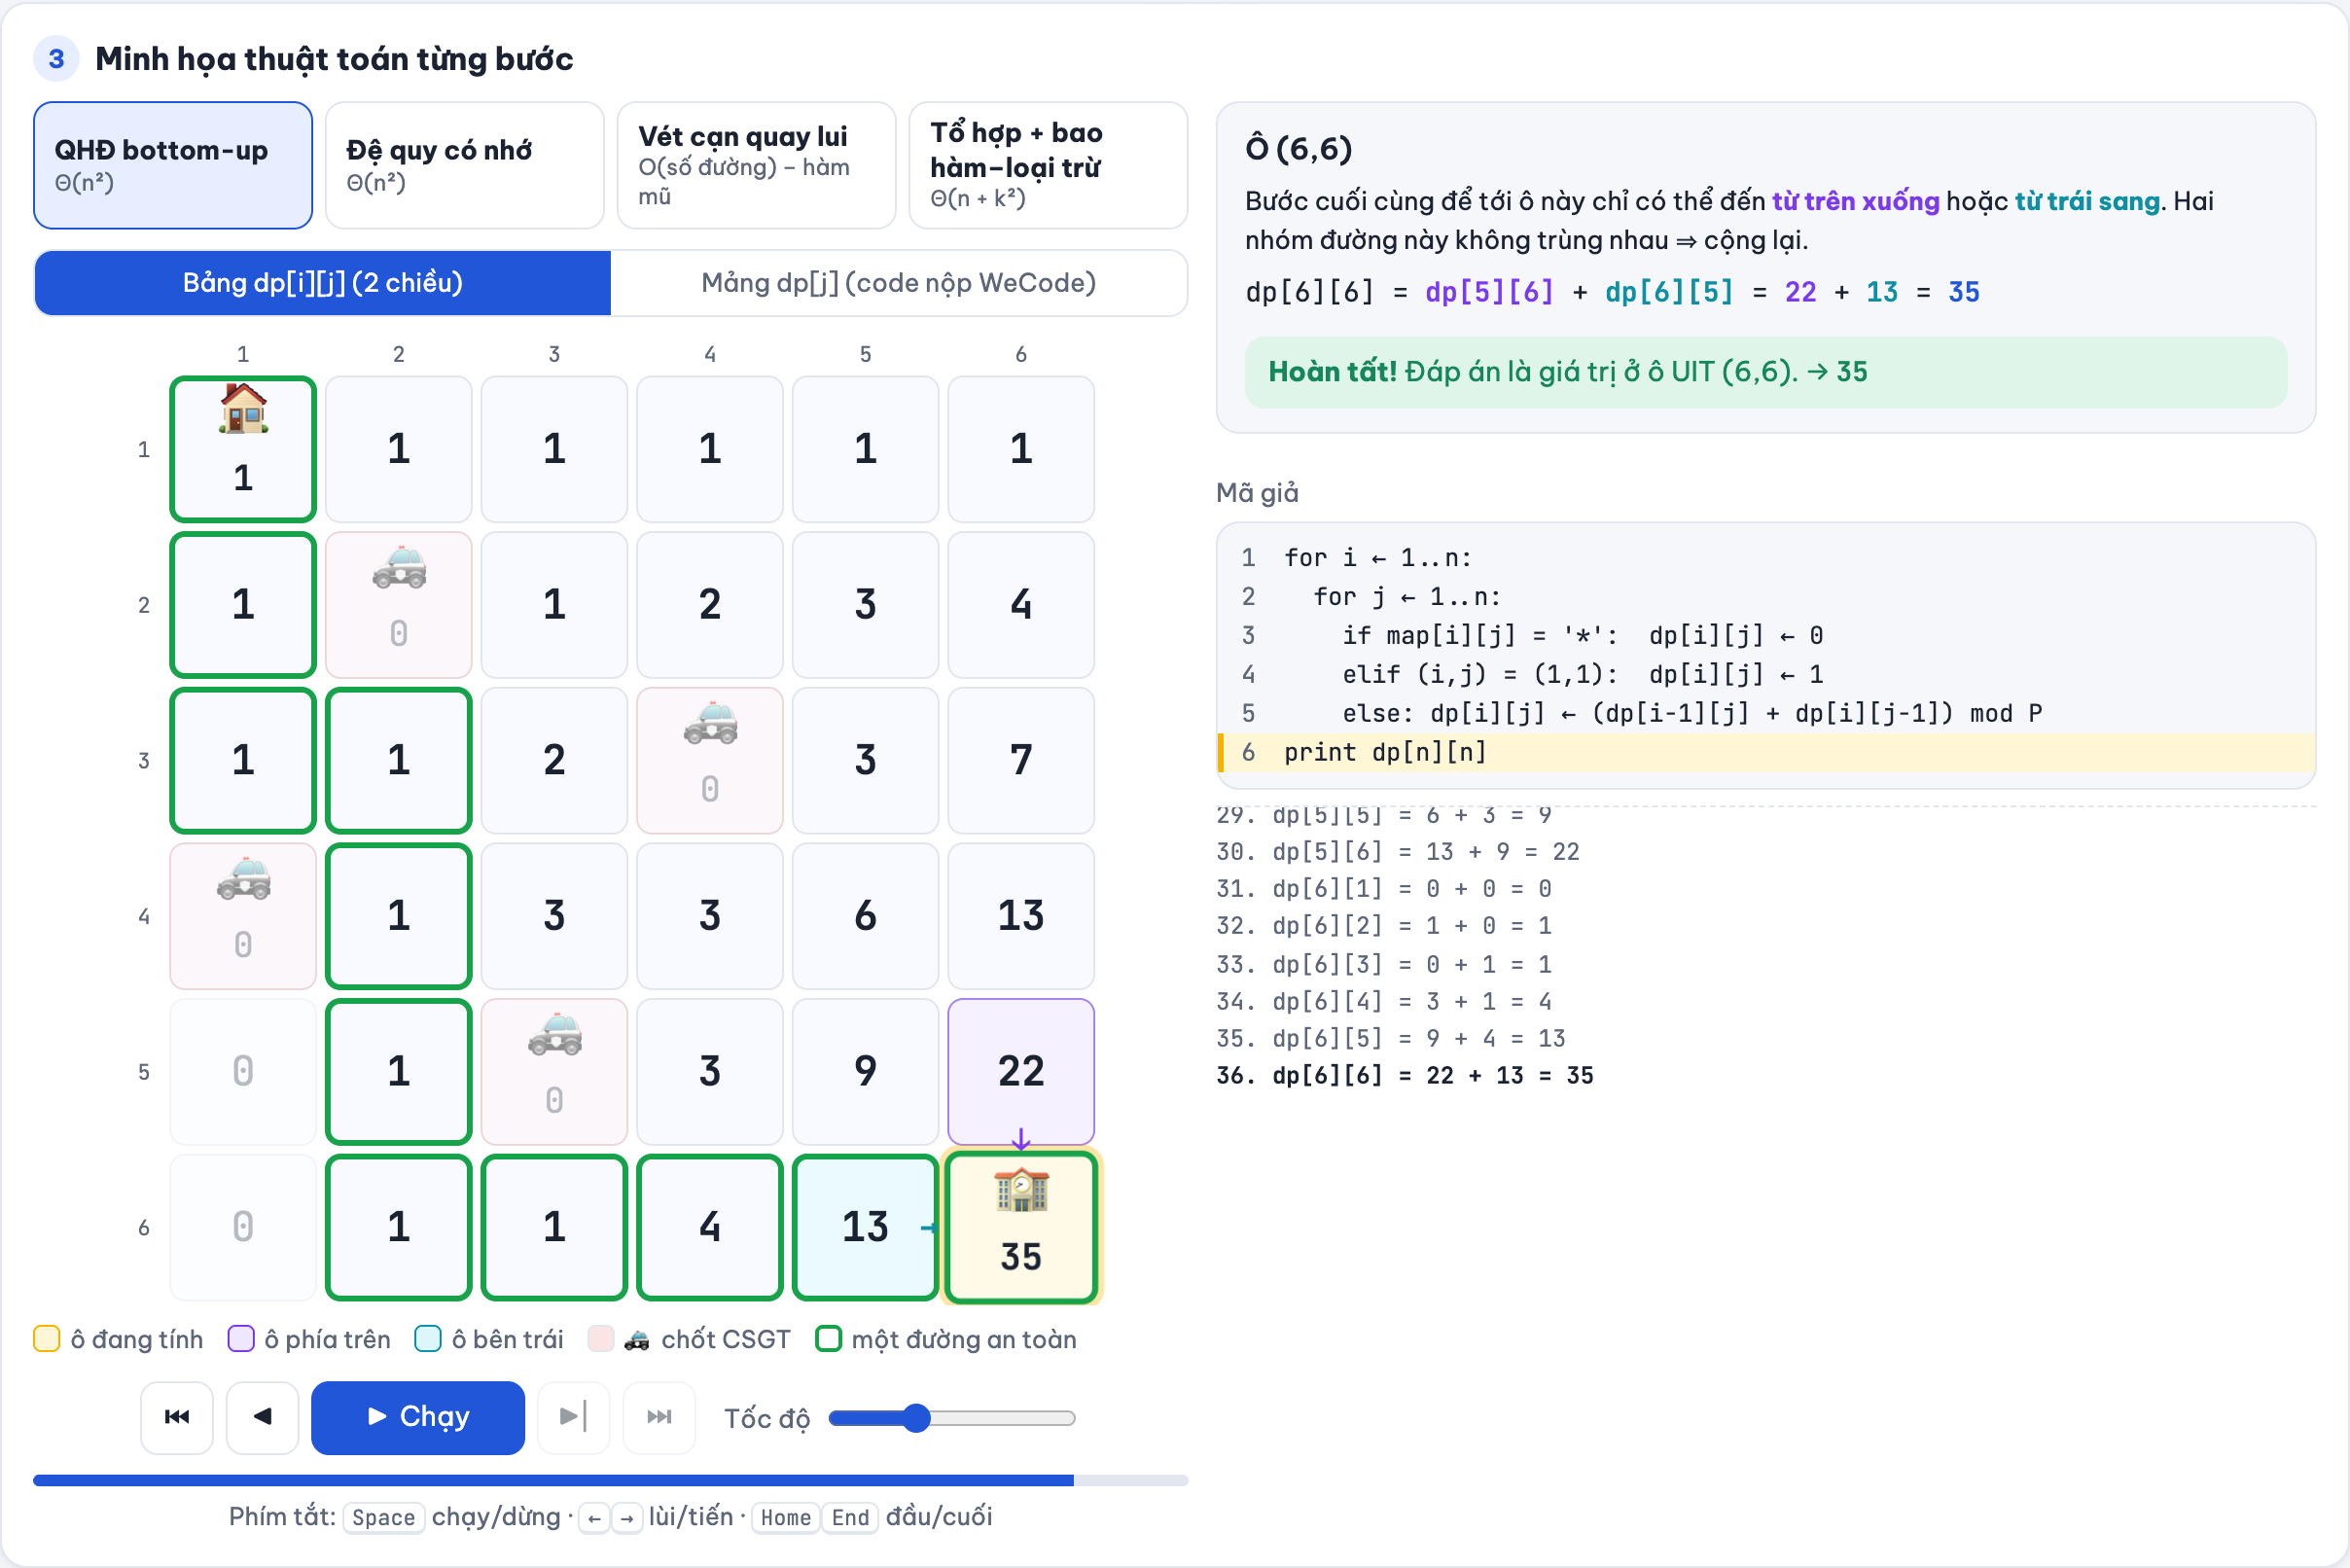
\includegraphics[width=0.95\linewidth]{img/path.png}
\caption{Demo khi tới ô $(6,6)$: $dp[6][6]=dp[5][6]+dp[6][5]=22+13=35$; viền xanh lá là một đường an toàn ngẫu nhiên, các ô mờ không nằm trên đường an toàn nào.}\label{fig:dp}\end{figure}
\begin{figure}[H]\centering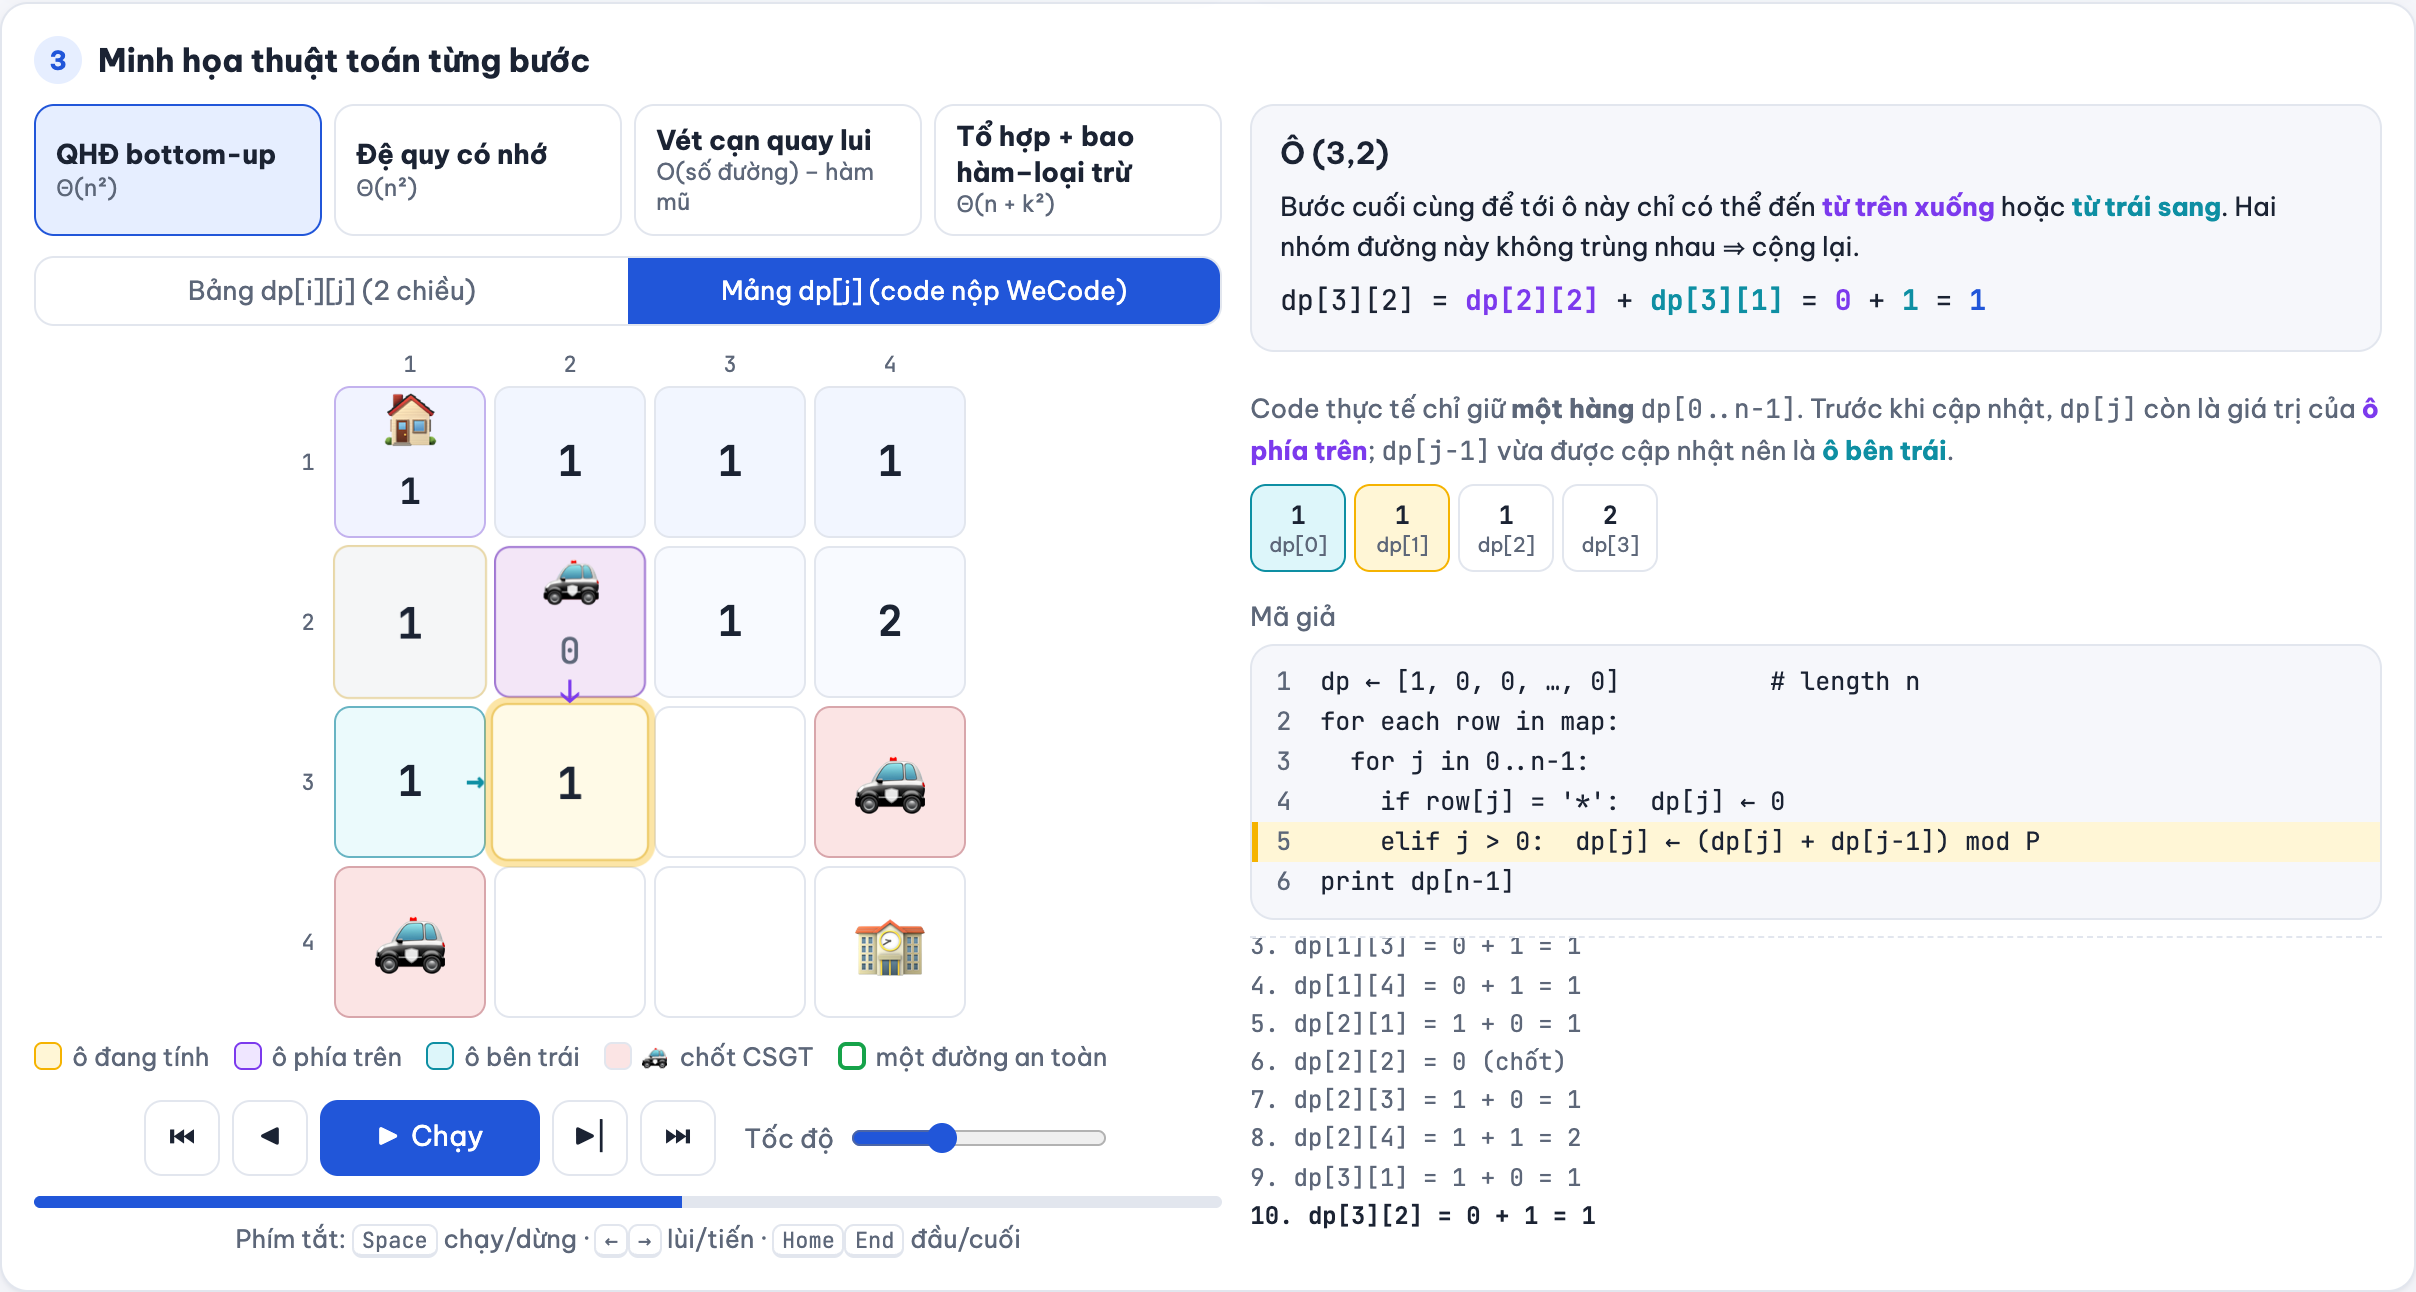
\includegraphics[width=0.95\linewidth]{img/step_1d.png}
\caption{Chế độ mảng 1 chiều: ô vàng là $dp[j]$ đang cập nhật (đang giữ giá trị ô trên), ô xanh là $dp[j-1]$ (ô trái).}\end{figure}

\section{Đệ quy có nhớ}
Lời gọi bắt đầu từ $f(6,6)$ và đi ngược về KTX. Trên ví dụ này có \textbf{\ExCalls{} lời gọi}, trong đó \textbf{\ExHits{} lần dùng lại bảng nhớ}; ngăn xếp sâu tối đa \ExDepth{} tầng. Mỗi lần ``dùng lại'' là một cây con đệ quy mà vét cạn phải duyệt lại từ đầu. Demo tô tím các ô đang nằm trên ngăn xếp gọi, các ô đã có trong bảng nhớ hiện giá trị (Hình~\ref{fig:memo}).
\begin{figure}[H]\centering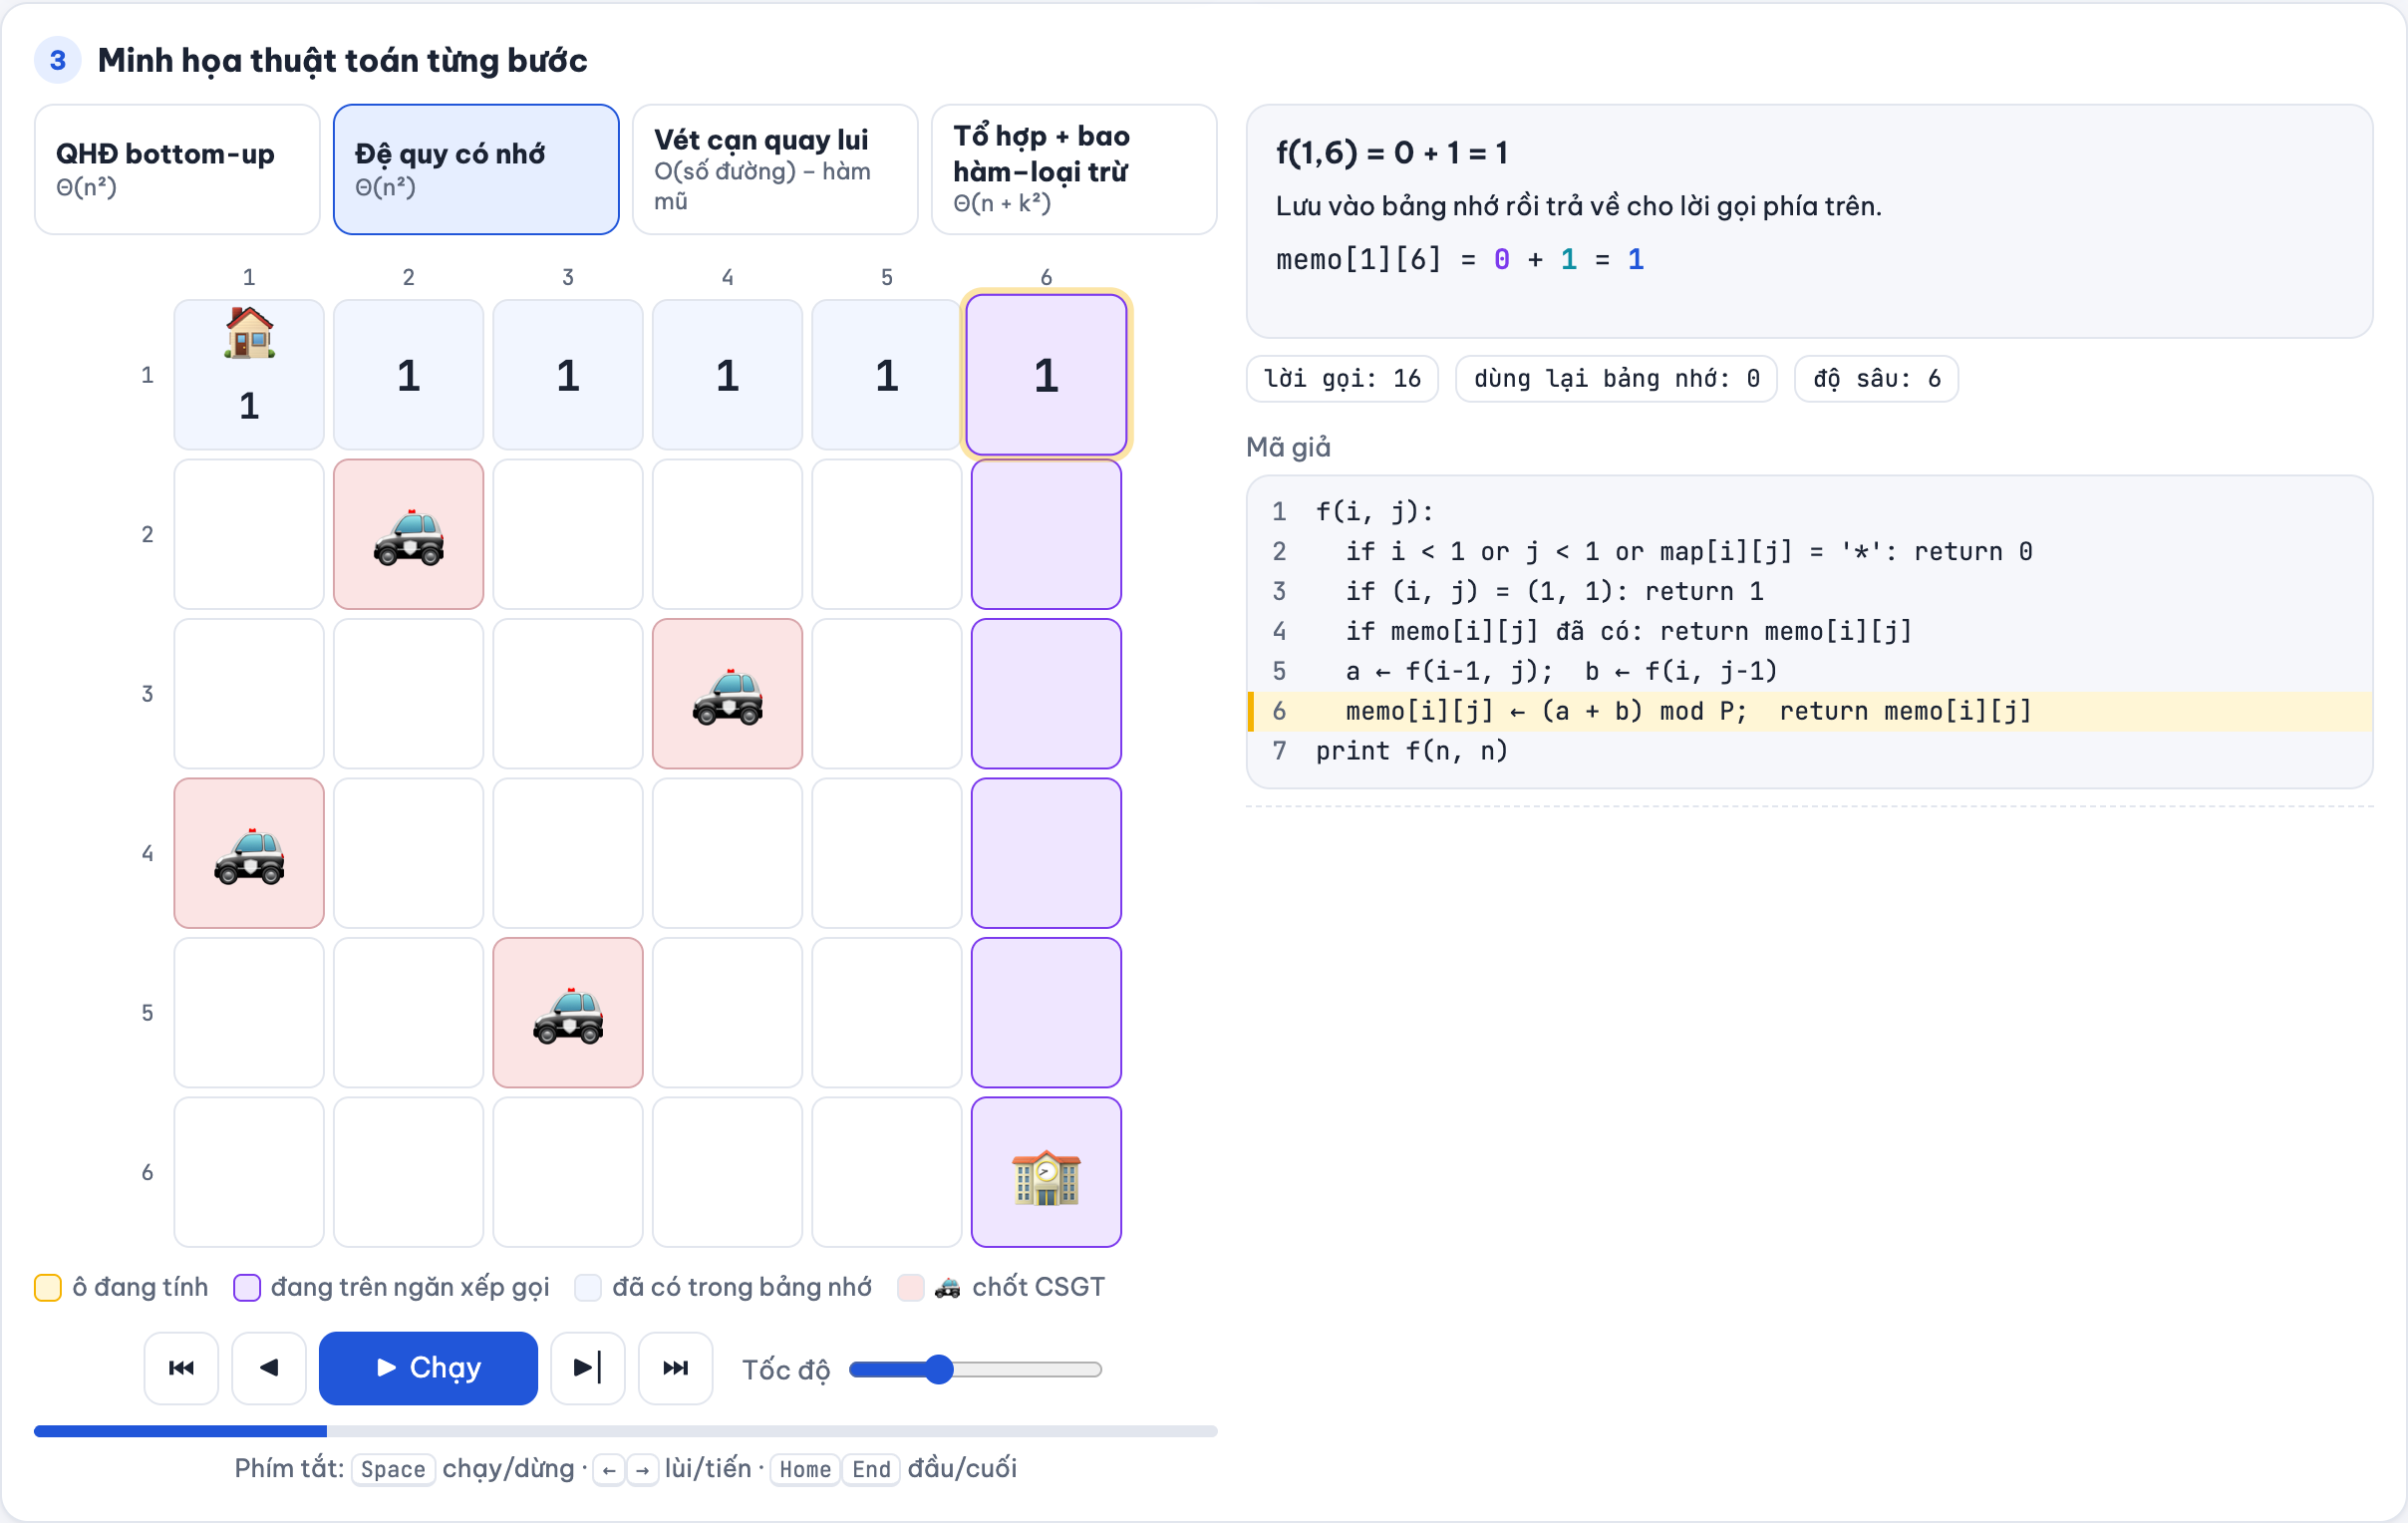
\includegraphics[width=0.95\linewidth]{img/algo_memo.png}
\caption{Đệ quy có nhớ: ngăn xếp gọi (tím), ô đang xét (vàng), mã giả tô dòng đang chạy, bộ đếm lời gọi, số lần dùng lại và độ sâu.}\label{fig:memo}\end{figure}

\section{Vét cạn quay lui}
DFS liệt kê đủ 35 đường với \textbf{\ExOpsBrute{} lời gọi}, gấp khoảng 4 lần QHĐ dù lưới chỉ $6\times6$. Khoảng cách này tăng theo hàm mũ (Chương~8). Demo vẽ đường đang thử màu xanh lá, ô vàng là ô vừa tới, bộ đếm ``đường tìm được'' tăng mỗi khi chạm UIT (Hình~\ref{fig:brute}).
\begin{figure}[H]\centering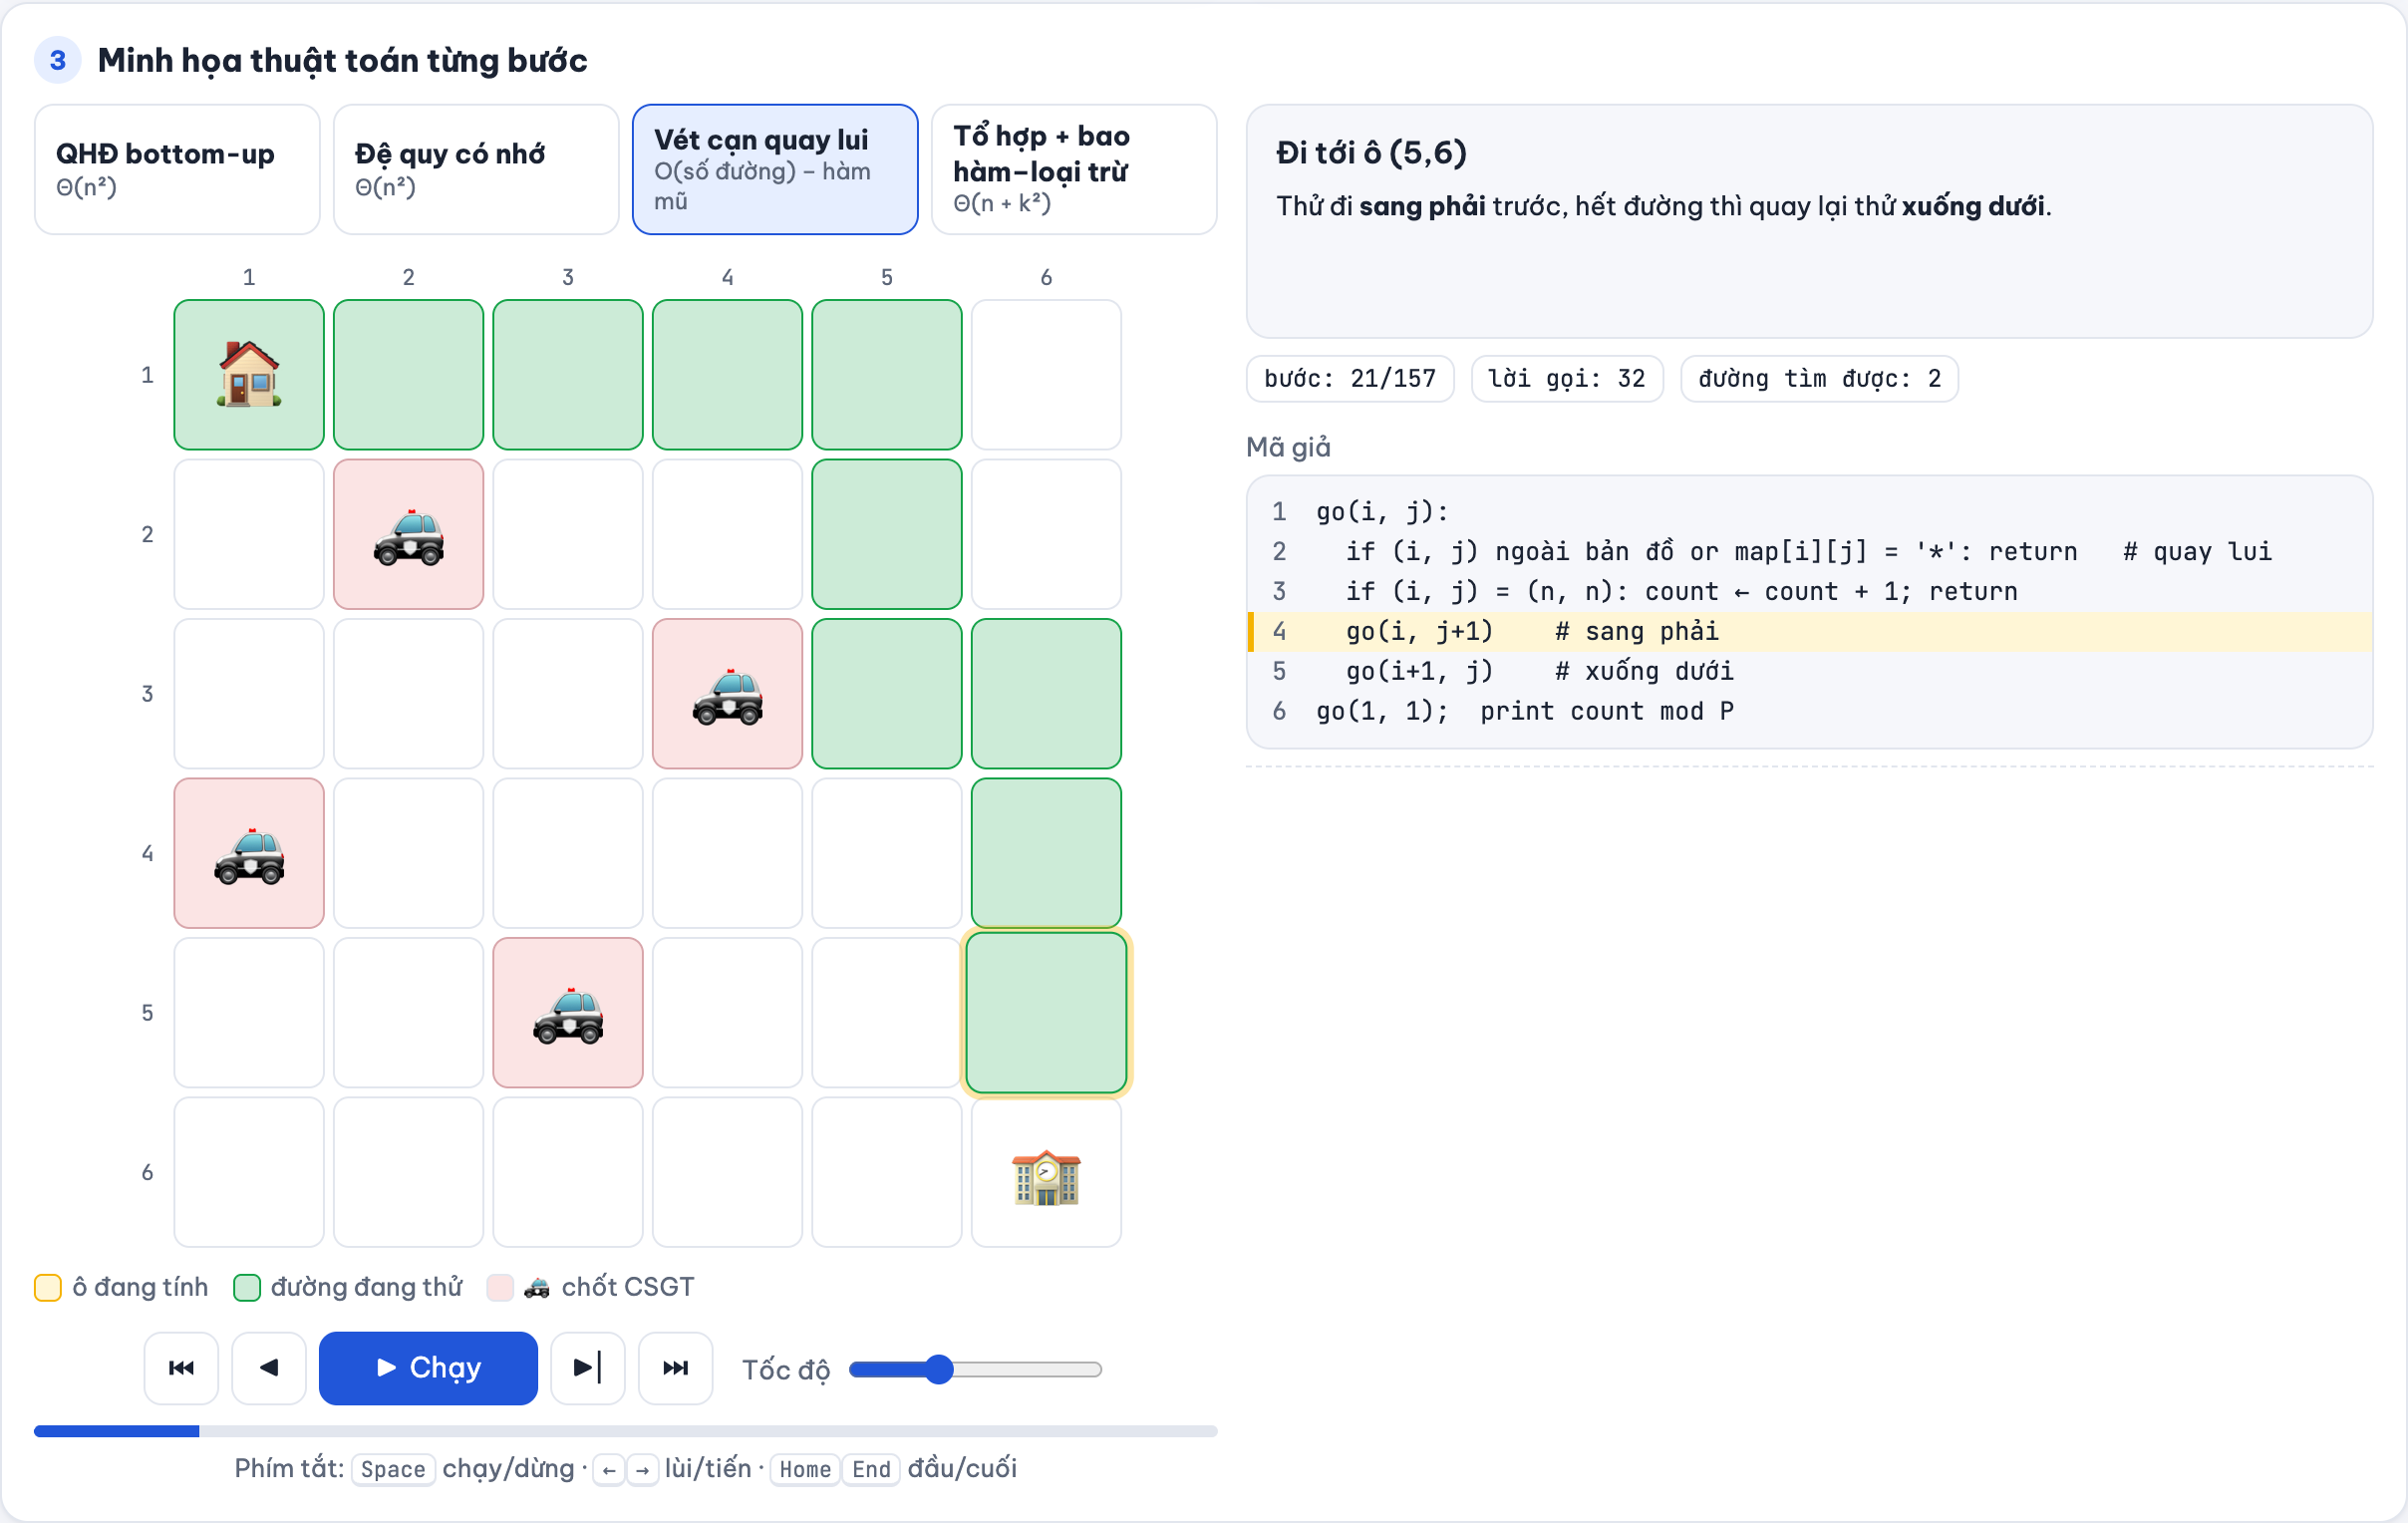
\includegraphics[width=0.95\linewidth]{img/algo_brute.png}
\caption{Vét cạn: đường đang thử, số lời gọi và số đường đã tìm được.}\label{fig:brute}\end{figure}

\section{Tổ hợp + bao hàm--loại trừ}
Bốn chốt sắp theo (hàng, cột): $\#1=(2,2)$, $\#2=(3,4)$, $\#3=(4,1)$, $\#4=(5,3)$, sau đó là UIT. Mỗi bước tính một giá trị $g$ (tọa độ trong $\binom{\cdot}{\cdot}$ tính theo 0):
\ExIE
\noindent Ví dụ ở bước 4: trong 15 đường tới $(5,3)$ có $2\cdot4=8$ đường mà chốt đầu tiên gặp là \#1 và $1\cdot3=3$ đường mà chốt đầu tiên gặp là \#3, nên $g_4=15-8-3=4$. Chốt \#2 nằm bên phải $(5,3)$ nên không tính. Chỉ cần \ExOpsIe{} thao tác.
\begin{figure}[H]\centering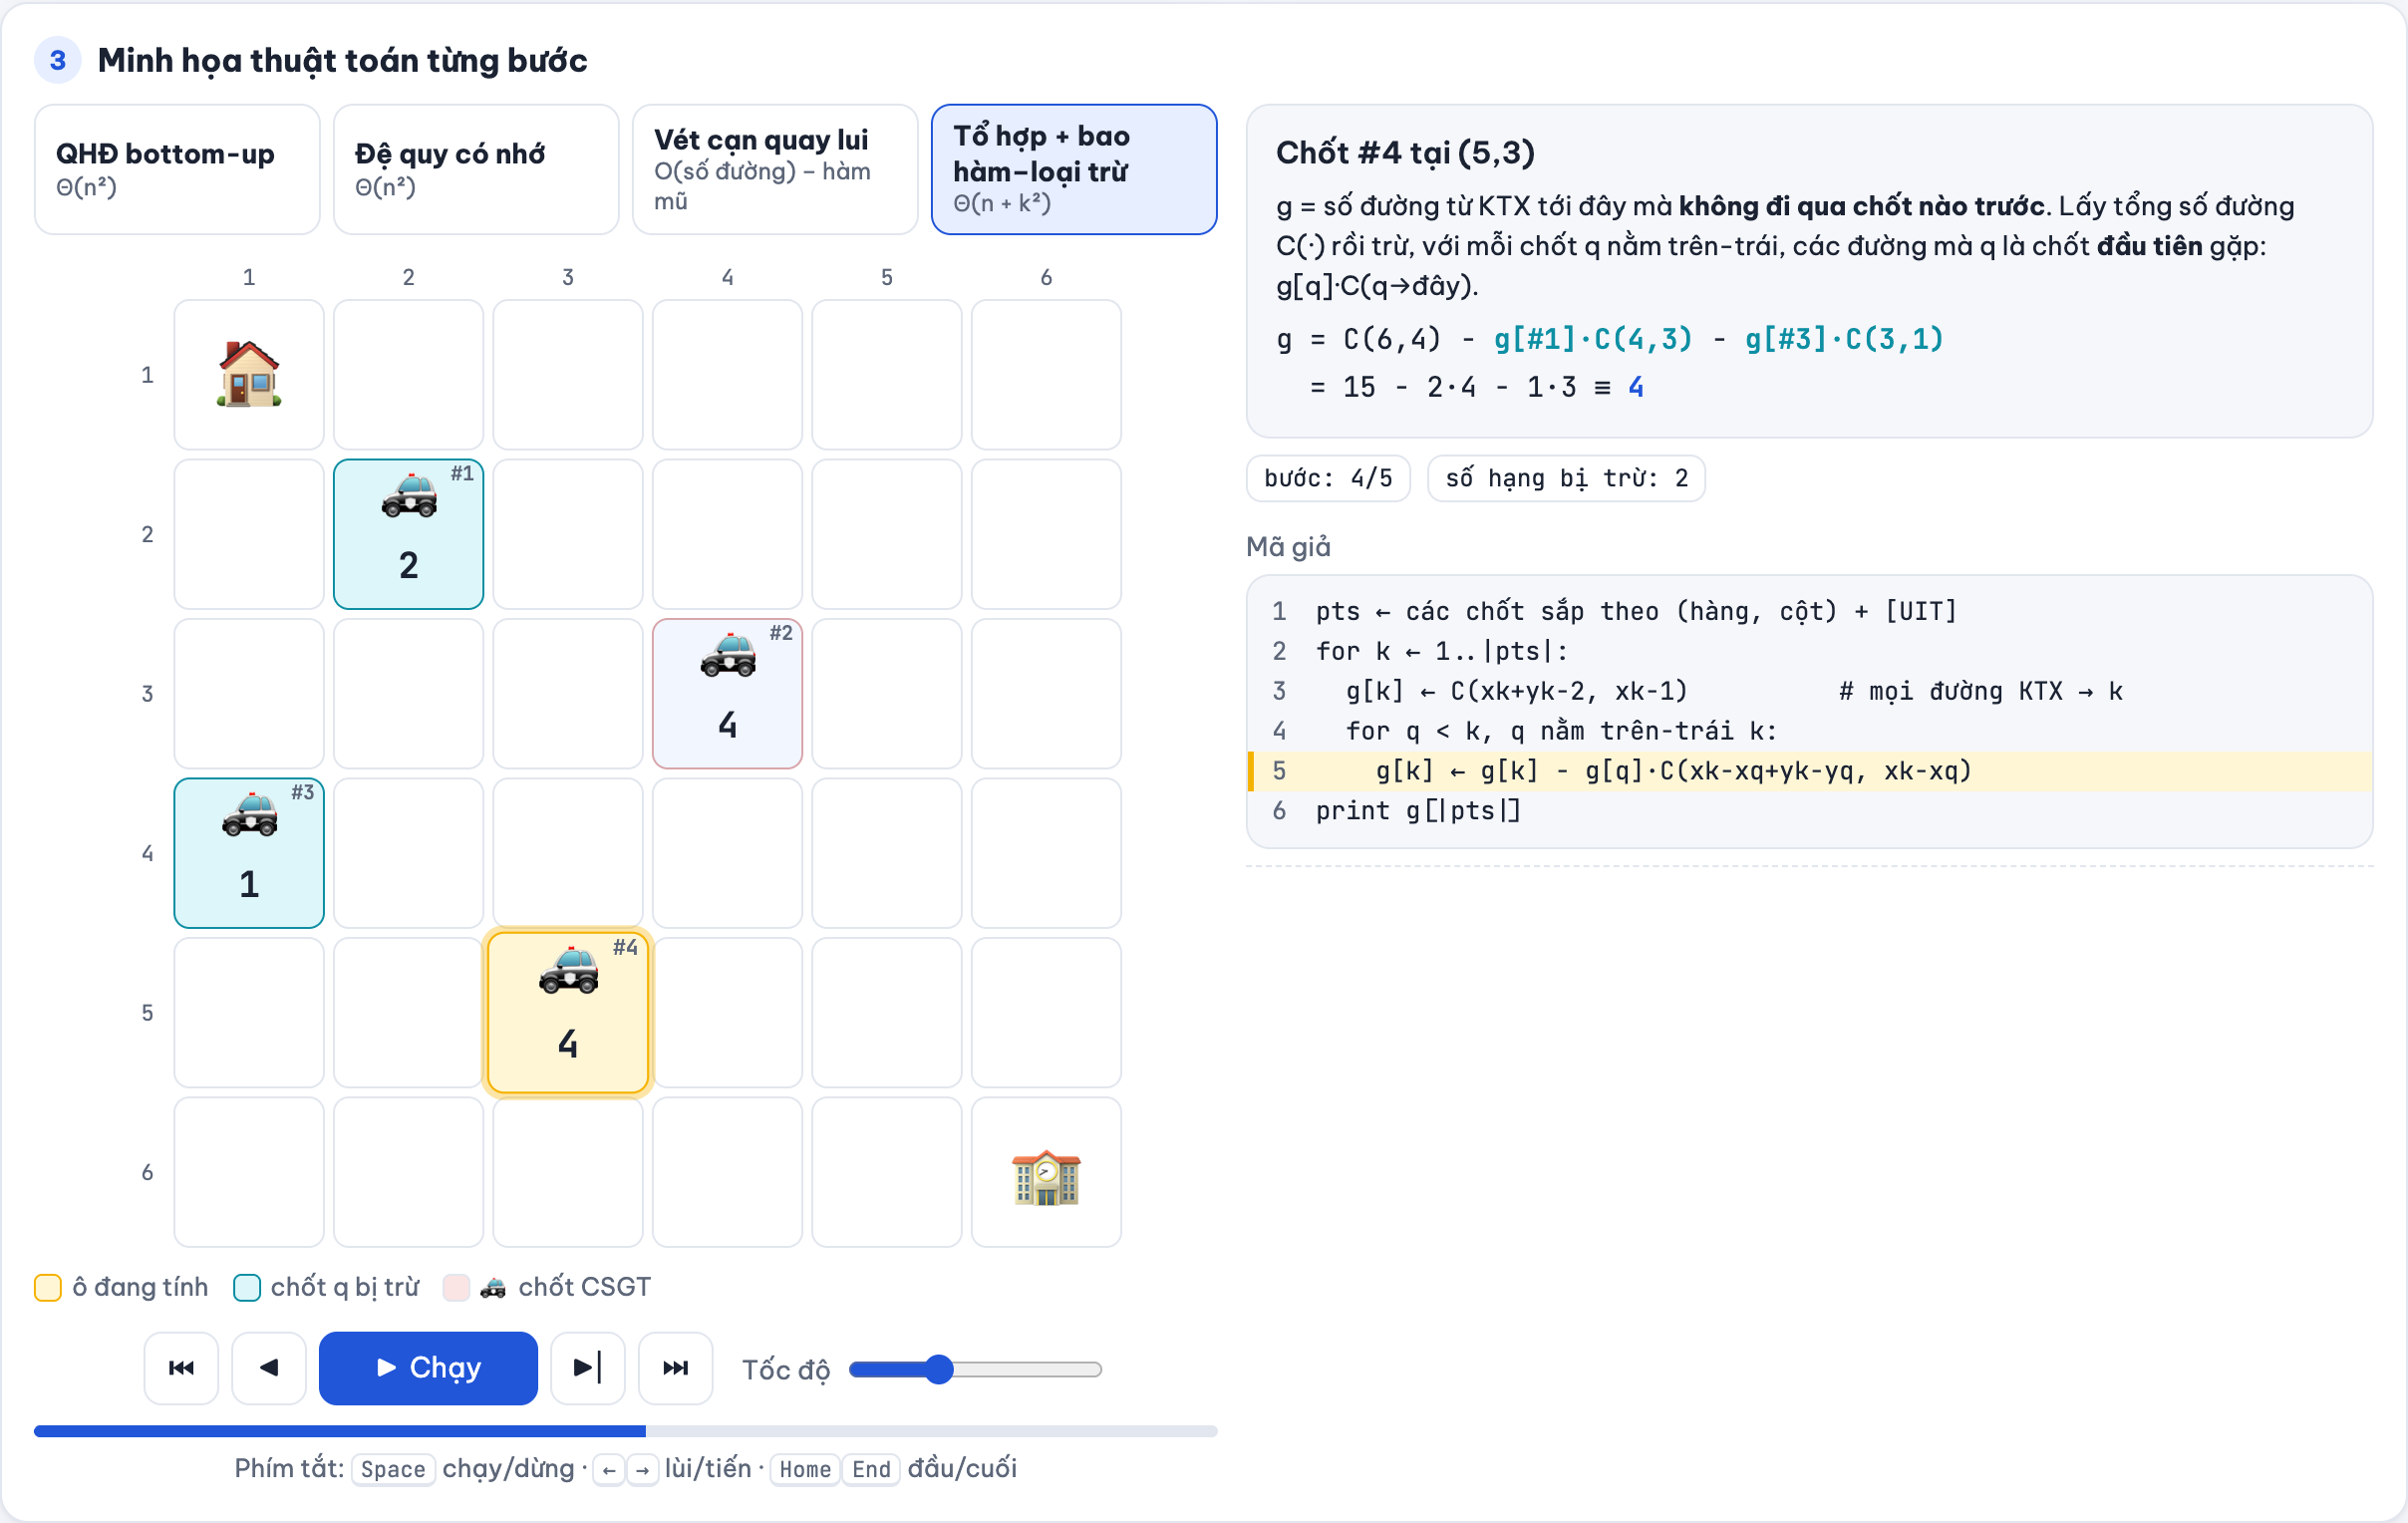
\includegraphics[width=0.95\linewidth]{img/algo_ie.png}
\caption{Bao hàm--loại trừ trên demo: chốt đang xét (vàng), các chốt bị trừ (xanh), công thức với số cụ thể.}\end{figure}

% =====================================================
\chapter{Quá trình thiết kế và xây dựng}
\section{Công cụ sử dụng}
\begin{itemize}
  \item \textbf{AI:} Claude Code (mô hình Claude Opus 5.5 của Anthropic), chạy trong ứng dụng Claude desktop. Công cụ này đọc/ghi file trong thư mục môn học, chạy lệnh trên máy và điều khiển trình duyệt để tự kiểm tra giao diện.
  \item \textbf{Ngôn ngữ, thư viện:} HTML/CSS/JavaScript thuần (không framework) cho demo; Python 3 cho lời giải nộp bài, sinh test và chạy test; Node.js để chạy lõi JS khi kiểm thử.
  \item \textbf{Công cụ phụ trợ:} Playwright + Google Chrome (chụp ảnh, quay video tự động), ffmpeg (ghép video), Tectonic (biên dịch \LaTeX), Git + GitHub Pages (lưu trữ, đăng demo).
  \item \textbf{Tra cứu:} em không tra Google; chỉ dùng AI và tài liệu môn học (transcript, slide).
\end{itemize}

\section{Tiến trình theo giai đoạn}
Toàn bộ quá trình diễn ra trong một phiên làm việc dài với Claude Code, từ ngày 05/10 đến 08/10/2026. Bảng~\ref{tab:prompts} liệt kê nguyên văn các prompt (phần dán dài được rút gọn). Mỗi giai đoạn dưới đây trình bày: mục tiêu, AI đã làm gì, vấn đề gặp phải, cách giải quyết, và em đã kiểm tra hoặc chỉnh sửa gì.

\subsection*{Giai đoạn 0 -- Xác định yêu cầu (prompt 1, 2)}
Em nhờ AI đọc 10 file phụ đề (\texttt{.vtt}) của các buổi học để tìm chỗ cô giao bài tập lớn. AI tìm được đoạn ở Buổi 8 (khoảng phút 12--22 và cuối buổi). \emph{Vấn đề:} phụ đề tự động ghi sai nhiều chữ (``WeChode'', ``distra'' = Dijkstra, ``một cái chuột cần phải nộp''). \emph{Cách xử lý:} em tự tóm tắt yêu cầu rồi nhờ AI đối chiếu lại với transcript. AI chỉ ra mốc thời gian sai và việc ``nộp source code'' chỉ là suy luận (vì câu gốc bị ghi sai), không phải lời nguyên văn của cô.

\subsection*{Giai đoạn 1 -- Chốt yêu cầu sản phẩm (prompt 3, 4)}
Thay vì bắt AI làm ngay, em yêu cầu AI \emph{đặt câu hỏi trước}. AI hỏi 17 câu về bài toán, công nghệ, mức độ minh họa, report, video. Em trả lời: chọn bài này (kèm đề và code Python đã Accepted), web, minh họa từng bước cho \emph{người mới học}, có nhập tay + sinh ngẫu nhiên + validate, song ngữ, report \LaTeX\ trung thực, thuật toán ``AI đề xuất -- em kiểm chứng''. Việc này giúp sản phẩm đúng ý ngay từ đầu.

\subsection*{Giai đoạn 2 -- Lõi thuật toán và kiểm chứng}
AI tách lõi thuật toán ra file \texttt{core.js} để dùng chung cho trình duyệt và cho Node.js khi test, rồi viết bộ test so sánh với vét cạn. Kết quả lần đầu: 307/307 bản đồ ngẫu nhiên khớp; $n=1000$ không có chốt ra $965\,601\,742 = \binom{1998}{999}\bmod p$. Em kiểm tra lại bằng cách chạy tay ví dụ $4\times4$ (ra 3) và đối chiếu với lời giải WeCode của mình.

\subsection*{Giai đoạn 3 -- Thiết kế giao diện}
Các quyết định thiết kế (AI đề xuất, em duyệt):
\begin{itemize}
  \item Bố cục 6 khối theo đúng mạch đọc: \emph{Bài toán $\to$ Nhập dữ liệu $\to$ Minh họa $\to$ Kết quả $\to$ So sánh $\to$ Phân tích}.
  \item \textbf{Mã màu thống nhất} cho toàn bộ demo, report và video: vàng = ô đang tính, tím = ô phía trên / ngăn xếp gọi, xanh ngọc = ô bên trái / chốt bị trừ, đỏ = chốt, xanh lá = đường đi.
  \item Mỗi bước có ba lớp thông tin: hình trên lưới, câu giải thích kèm công thức có số cụ thể, và dòng mã giả đang chạy. Người mới học có thể nối ``hình'' với ``code''.
  \item Hai chế độ xem cho QHĐ: bảng 2 chiều (dễ hiểu) và mảng 1 chiều (đúng code nộp bài).
  \item Lưới lớn ($n>16$) không chạy hoạt hình từng ô (không đọc được) mà hiện bản đồ nhiệt.
\end{itemize}
\textbf{Vấn đề gặp phải khi AI tự mở demo trên trình duyệt để kiểm tra, và cách sửa:}
\begin{center}
\begin{tabular}{p{6.6cm} p{7.6cm}}
\toprule
\textbf{Lỗi phát hiện} & \textbf{Nguyên nhân / cách sửa}\\\midrule
Khoảng trống lớn dưới lưới & Thuộc tính \texttt{hidden} của canvas bị CSS \texttt{display:block} ghi đè; thêm \texttt{[hidden]\{display:none!important\}}.\\
Ô KTX/UIT bị biểu tượng che mất giá trị & Biểu tượng đặt ở giữa ô; đổi thành biểu tượng phía trên, số phía dưới.\\
Trên điện thoại trang bị tràn ngang (472px/375px) & Thanh chọn chế độ không xuống dòng; cho các nút co giãn, tính lại kích thước ô theo bề rộng.\\
Chuyển sang lưới lớn vẫn còn nhật ký của lưới cũ & Xóa nhật ký và mã giả khi vào chế độ bản đồ nhiệt.\\
\bottomrule
\end{tabular}
\end{center}

\subsection*{Giai đoạn 4 -- Video demo (nhiều vòng góp ý)}
\begin{enumerate}
  \item \textbf{Vòng 1:} AI viết script Playwright điều khiển Chrome theo kịch bản và thuyết minh bằng giọng ``Linh'' của macOS. \emph{Lỗi:} video bị một dải xám ở đáy. AI dùng một trang thử có dải màu chuyển để đo, phát hiện Chrome headless chỉ vẽ $\approx$ (chiều cao $-$ 86px), bèn cắt video và đẩy phụ đề lên.
  \item \textbf{Vòng 2:} em nhận xét giọng đọc ``nghe kinh quá''. AI đổi sang giọng neural tiếng Việt (thư viện \texttt{edge-tts}). \emph{Lỗi:} lần gọi đầu báo \texttt{NoAudioReceived} do mạng chập chờn; AI thêm cơ chế thử lại.
  \item \textbf{Vòng 3:} em muốn video không lời mà người xem vẫn hiểu. AI làm chế độ ``rọi đèn'' (làm tối mọi thứ trừ vùng đang nói tới), thẻ tiêu đề chia chương, phụ đề hiện theo độ dài chữ.
  \item \textbf{Vòng 4:} em góp ý video chậm và cần con trỏ chỉ vào vùng khoanh. AI tăng tốc (khoảng 17 ký tự/giây, người xem có thể tạm dừng) và thêm con trỏ mũi tên di chuyển tới vùng rọi sáng, có hiệu ứng ``chạm''.
\end{enumerate}
Bản nộp là video không lời (\texttt{2\_VideoDemo/demo.mp4}), đúng với hướng dẫn cô cho phép ``hiện text hoặc video không lời''.

\subsection*{Giai đoạn 5 -- Triển khai}
AI tạo kho mã công khai trên GitHub và bật GitHub Pages; demo chạy online tại \demo. AI mở trang online để kiểm tra: trang tự chuyển tới ứng dụng và cho đúng đáp án ví dụ.

\subsection*{Giai đoạn 6 -- Mở rộng theo yêu cầu cập nhật của cô (prompt 8, 9)}
Em dán yêu cầu mới của cô. AI liệt kê các điểm còn thiếu (bộ testcase riêng, cấu trúc 4 thư mục, nhiều mục report mới, tiêu chí sáng tạo) và hỏi em chọn hướng mở rộng; em chọn \textbf{so sánh 4 thuật toán}. Vấn đề kỹ thuật và cách giải quyết:
\begin{itemize}
  \item \textbf{Đệ quy có nhớ với $n=1000$:} đệ quy thường sâu 2000 tầng, có nguy cơ tràn stack. AI chuyển sang ngăn xếp tường minh với các ``giai đoạn'' của mỗi khung gọi.
  \item \textbf{Nhân mod trong JavaScript:} tích hai số $\approx10^9$ vượt $2^{53}$ nên mất chính xác. AI viết \texttt{mulmod} tách 16 bit.
  \item \textbf{Bao hàm--loại trừ chậm khi nhiều chốt} ($k=10^5\Rightarrow10^{10}$ phép tính, treo trình duyệt). AI giới hạn $k\le4000$ và hiển thị lý do bỏ qua. Đây cũng là một kết luận so sánh quan trọng.
  \item \textbf{Vét cạn bùng nổ:} giới hạn số lời gọi; phần minh họa chỉ chạy các bước đầu và báo tổng số lời gọi thực tế.
  \item \textbf{Chú thích biểu đồ bị tràn khung:} chuyển chú thích từ SVG ra HTML.
\end{itemize}
Kiểm chứng: 4 cách giải được so với nhau trên 3000 bản đồ ngẫu nhiên ($n\le 9$) và với đáp án độc lập trên toàn bộ 103 testcase (Chương~7, 8). Em kiểm tra lại bằng tay bước bao hàm--loại trừ của chốt \#4 ($15-8-3=4$) và đối chiếu với bảng $dp$.

\section{Danh sách prompt đã dùng}
\begin{longtable}{>{\centering\arraybackslash}p{0.5cm} >{\raggedright\arraybackslash}p{6.1cm} >{\raggedright\arraybackslash}p{6.9cm}}
\caption{Các prompt và kết quả nhận được}\label{tab:prompts}\\
\toprule
\# & \textbf{Prompt của em} & \textbf{Kết quả AI trả về}\\\midrule\endhead
1 & \textit{``check tài liệu trong docs đọc transcript và cho tôi biết ở buổi máy, mốc thời gian nào cô yêu cầu làm bài tập lớn, nội dung yêu cầu là gì''} & Xác định Buổi 8, trích yêu cầu kèm mốc thời gian.\\\midrule
2 & Dán bản tóm tắt em tự viết, hỏi \textit{``như vậy đúng chưa?''} & Xác nhận và sửa 4 điểm (mốc giờ, mục suy luận, việc về nhà thứ hai, ý ở Buổi 10).\\\midrule
3 & \textit{``\dots dựa vào những dữ liệu trên, hãy đưa ra những câu hỏi để giúp bạn có thể làm bài tập này.''} & 17 câu hỏi làm rõ yêu cầu.\\\midrule
4 & Trả lời 17 câu (dán đề, hình, code Python; chọn web, song ngữ, \LaTeX, \textit{``AI đề xuất rồi bạn kiểm chứng''}, \dots) & Lõi thuật toán, test vét cạn, giao diện, video, report bản đầu.\\\midrule
5 & \textit{``deploy github nhé, còn video lòng tiếng nghe kinh quá, có cách khác không''} & GitHub Pages; 3 phương án giọng đọc; em chọn giọng AI neural; hai bản giọng nữ/nam.\\\midrule
6 & \textit{``tôi muốn quay demo không lòng tiếng như người xem vẫn có thể hiểu thì làm sao ?''} & Video không lời: thẻ chương, rọi sáng, phụ đề theo tốc độ đọc.\\\midrule
7 & \textit{``tốc độ nên nhanh hơn 1 chút, nếu người xem muốn coi kỹ thì chỉ cần pause video, ở những chỗ khoanh vùng nên có thêm pointer dạng mũi tên hay ngón tay''} & Video nhanh hơn (3 phút $\to$ 2 phút 10 giây), con trỏ mũi tên và hiệu ứng chạm.\\\midrule
8 & Dán yêu cầu cập nhật của cô (đề bài, 4 thư mục nộp, nội dung report, tiêu chí đánh giá) & Phân tích chỗ thiếu; hỏi 4 câu (hướng mở rộng, lý do chọn bài, nguồn gốc code, có tra Google).\\\midrule
9 & Trả lời: so sánh 4 thuật toán; lý do: đã làm trên WeCode; code tự viết, Accepted; không tra Google & 3 thuật toán mới + minh họa, so sánh, benchmark; 103 testcase; cấu trúc 4 thư mục; report này.\\
\bottomrule
\end{longtable}

\section{Phân định phần việc của em và của AI}
\begin{itemize}
  \item \textbf{Em:} chọn bài toán; tự viết lời giải QHĐ 1 chiều và nộp đạt trên WeCode (Phụ lục A); quyết định đối tượng người dùng, phạm vi chức năng, hướng mở rộng; góp ý từng vòng (giọng đọc, tốc độ, con trỏ); kiểm tra kết quả: chạy tay các ví dụ, đọc lại công thức, xem demo và video.
  \item \textbf{AI:} đề xuất ba cách giải bổ sung cùng chứng minh, phân tích độ phức tạp; viết code giao diện, script sinh/chạy test, script quay video, bản thảo report; tự kiểm tra giao diện trên trình duyệt.
  \item \textbf{Nguyên tắc kiểm chứng:} không tin lập luận của AI một cách mặc nhiên. Mọi kết quả đều được đối chiếu với một phương pháp độc lập: vét cạn, số nguyên lớn không lấy dư, công thức $\binom{2n-2}{n-1}$, và chạy tay.
\end{itemize}

% =====================================================
\chapter{Thiết kế thực nghiệm}
\section{Cách xây dựng bộ testcase}
Bộ test nằm ở thư mục \texttt{3\_Testcase}, được sinh bằng \texttt{gen\_tests.py} với seed cố định (sinh lại y hệt). Mỗi test gồm file \texttt{.inp} đúng định dạng WeCode và file \texttt{.out} chứa đáp án. Demo mở được trực tiếp file \texttt{.inp} (nút ``Mở file .inp'').

\textbf{Đáp án được tính độc lập với các lời giải cần kiểm tra:} QHĐ 2 chiều bằng số nguyên lớn của Python, không lấy dư giữa chừng, chỉ lấy dư ở cuối. Ngoài ra:
\begin{itemize}
  \item mọi test $n\le 8$ được đối chiếu thêm với phép \emph{liệt kê từng đường};
  \item mọi bản đồ không có chốt được đối chiếu với công thức $\binom{2n-2}{n-1}$.
\end{itemize}
Script sẽ dừng ngay nếu có bất kỳ chênh lệch nào.

\section{Các nhóm testcase}
\begin{longtable}{p{2.6cm} c p{2.1cm} p{8.6cm}}
\toprule
\textbf{Nhóm} & \textbf{Số test} & \textbf{Kích thước} & \textbf{Mục đích, cách tạo}\\\midrule\endhead
01 Thông thường & 15 & $n=5..120$ & Bản đồ ngẫu nhiên, mật độ chốt 10--30\%, KTX và UIT để trống: trường hợp điển hình.\\\midrule
02 Biên & 27 & $n=1..1000$ & $n=1$ (trống/chốt); chốt tại KTX, tại UIT (cả với $n=1000$); chặn cả một hàng, một cột; chặn kín đường chéo phụ; chéo phụ chừa đúng 1 khe; hai ô kề KTX đều bị chặn; \textbf{toàn bộ 16 bản đồ $2\times2$}.\\\midrule
03 Nhỏ & 30 & $n=3..8$ & Mật độ 0--60\%, có test không giữ trống hai đầu; đều đối chiếu được bằng vét cạn.\\\midrule
04 Lớn & 10 & $n=500..1000$ & Chạm giới hạn $n=1000$, mật độ 0--45\% ($k$ tới 450\,000 chốt): kiểm tra thời gian và tràn số.\\\midrule
05 Đặc biệt & 10 & $n=9..1000$ & Không chốt ($n=10,20,100$; $n=20$ có đáp án thật vượt $10^9+7$); hành lang chỉ 1 đường; chỉ đi được trên viền (đúng 2 đường); bậc thang; bàn cờ (đáp án 0); mê cung răng cưa nhiều ngõ cụt; $n=200$ một khe; $n=1000$ rất ít chốt.\\\midrule
06 Không hợp lệ & 11 & -- & Rỗng; $n$ là chữ, số âm, số thực; $n=0$; $n=1001$; thiếu dòng; thừa dòng; dòng ngắn; dòng dài; ký tự lạ. Đáp án là \emph{loại lỗi} mà demo phải báo.\\
\bottomrule
\end{longtable}

\section{Lập luận về độ bao phủ}
\begin{itemize}
  \item \textbf{Theo cấu trúc lời giải:} có test để ô $(1,1)$ hoặc $(n,n)$ bị chặn (nhánh trả 0), test chỉ có cạnh trên/cạnh trái (nhánh $i=1$, $j=1$), test chốt ``đổ bóng'' làm cả vùng bằng 0, test đáp án vượt modulo.
  \item \textbf{Theo kích thước:} từ $n=1$ tới $n=1000$. Riêng $n=2$ được vét toàn bộ $2^4$ khả năng.
  \item \textbf{Theo mật độ chốt:} 0\% tới 60\%, cả bản đồ ngẫu nhiên lẫn bản đồ có cấu trúc (đường chéo, hành lang, viền, mê cung, bàn cờ).
  \item \textbf{Theo đặc tính từng thuật toán:} test rất ít chốt (bao hàm--loại trừ có lợi), test rất nhiều chốt (bao hàm--loại trừ bất lợi), test nhiều đường (vét cạn bất lợi), test mê cung (đệ quy có nhớ chỉ đi một phần lưới).
  \item \textbf{Ngoài định dạng:} 11 kiểu input sai.
\end{itemize}

\section{Quy trình chạy}
Lệnh \texttt{python3 3\_Testcase/run\_tests.py} chạy: (a) lời giải nộp WeCode (Python), so khớp đầu ra với \texttt{.out}; (b) cả 4 thuật toán trong \texttt{core.js} của demo (qua Node.js), đo thời gian và số thao tác; (c) bộ kiểm tra input của demo trên nhóm 06. Kết quả ghi ra \texttt{3\_Testcase/ket\_qua/}. Máy chạy: MacBook (Apple Silicon), Python 3.13, Node.js 24.

% =====================================================
\chapter{Đánh giá}
\section{Tính đúng đắn}
\begin{center}
\begin{tabular}{lccccc}
\toprule
\textbf{Nhóm} & \textbf{Số test} & \textbf{$n$} & \textbf{Đạt} & \textbf{Vét cạn} & \textbf{Bao hàm--loại trừ}\\
 & & & & \textit{chạy được} & \textit{chạy được}\\\midrule
Thông thường & 15 & 5--120 & 15/15 & 7/15 & 15/15\\
Biên & 27 & 1--1000 & 27/27 & 26/27 & 27/27\\
Nhỏ & 30 & 3--8 & 30/30 & 30/30 & 30/30\\
Lớn & 10 & 500--1000 & 10/10 & 1/10 & 1/10\\
Đặc biệt & 10 & 9--1000 & 10/10 & 5/10 & 10/10\\
Không hợp lệ & 11 & -- & 11/11 & -- & --\\\midrule
\textbf{Tổng} & \textbf{103} & & \textbf{103/103} & & \\
\bottomrule
\end{tabular}
\end{center}
``Đạt'' nghĩa là lời giải Python \emph{và mọi thuật toán chạy được} đều cho đúng đáp án; với nhóm 06 là demo báo đúng loại lỗi. ``Không chạy được'' là chủ động bỏ qua do vượt giới hạn (vét cạn quá $5\cdot10^7$ lời gọi; bao hàm--loại trừ quá 4000 chốt). Đây là \emph{giới hạn của phương pháp}, không phải kết quả sai. Đáng chú ý: vét cạn vẫn chạy được một test lớn ($n=1000$, mật độ 45\%) vì chốt dày làm hầu hết các hướng bị chặn sớm.

\section{Thời gian thực hiện}
\begin{center}
\begin{tabular}{lrrrrl}
\toprule
\textbf{Test (nhóm 04)} & \textbf{$k$} & \textbf{Python} & \textbf{Đệ quy nhớ} & \textbf{Bottom-up} & \textbf{Bao hàm--loại trừ}\\
 & & (ms) & (ms) & (ms) & \\\midrule
$n=1000$, 0\% & 0 & 156 & 50.8 & 5.2 & 2.9 ms\\
$n=1000$, 1\% & 10\,164 & 166 & 51.8 & 5.3 & bỏ qua\\
$n=1000$, 10\% & 100\,387 & 171 & 40.0 & 5.1 & bỏ qua\\
$n=1000$, 30\% & 299\,905 & 96 & 1.8 & 4.2 & bỏ qua\\
$n=1000$, 45\% & 450\,365 & 86 & 0.1 & 5.3 & bỏ qua\\
\bottomrule
\end{tabular}
\end{center}
Thời gian Python bao gồm cả khởi động trình thông dịch và đọc 1 triệu ký tự. Các cột JS chỉ đo phần thuật toán. Nhận xét:
\begin{itemize}
  \item QHĐ bottom-up ổn định nhất ($\approx5$ ms với mọi mật độ), đúng với $\Theta(n^2)$.
  \item Đệ quy có nhớ chậm hơn khoảng 10 lần khi bản đồ thông thoáng (chi phí quản lý ngăn xếp). Nhưng khi chốt dày nó gần như tức thì, vì chỉ gọi tới những ô thực sự tới được UIT. Đây là ưu điểm của cách top-down.
  \item Bao hàm--loại trừ thắng tuyệt đối khi không có chốt (2.9 ms, chỉ $\approx2000$ thao tác so với $10^6$), nhưng không dùng được khi có hàng nghìn chốt.
\end{itemize}

\begin{figure}[H]\centering
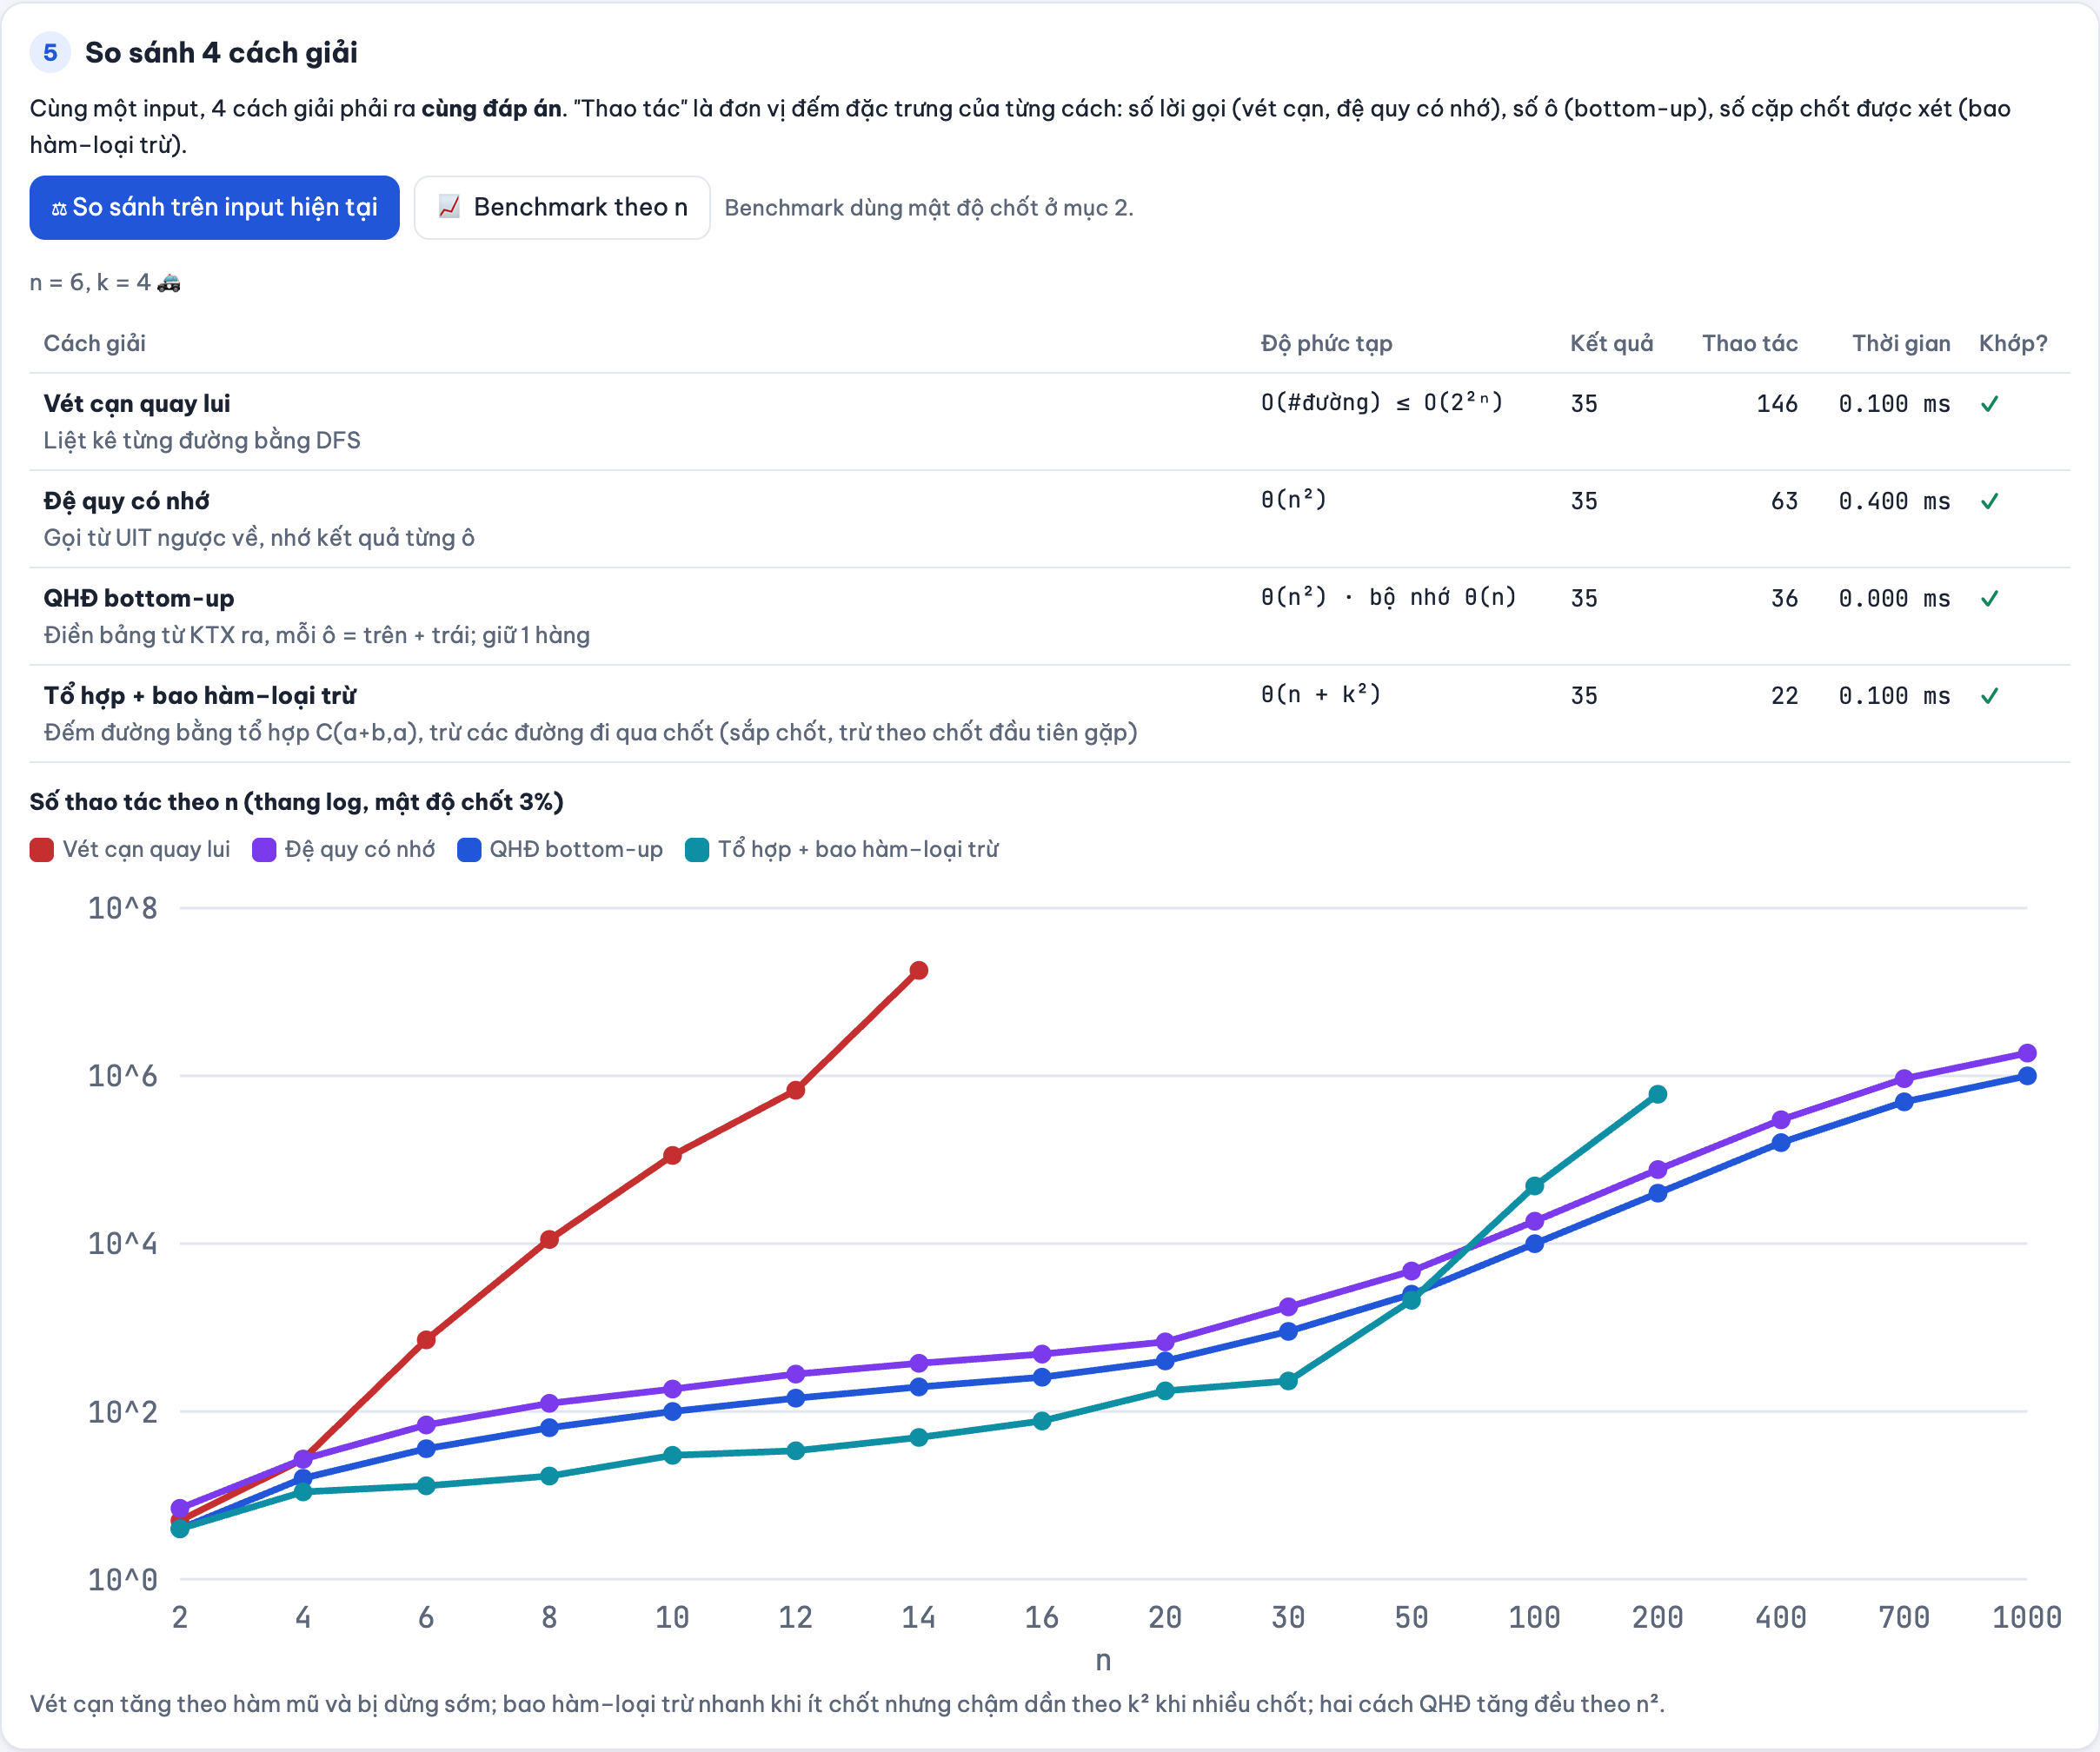
\includegraphics[width=0.49\linewidth]{img/compare.png}\hfill
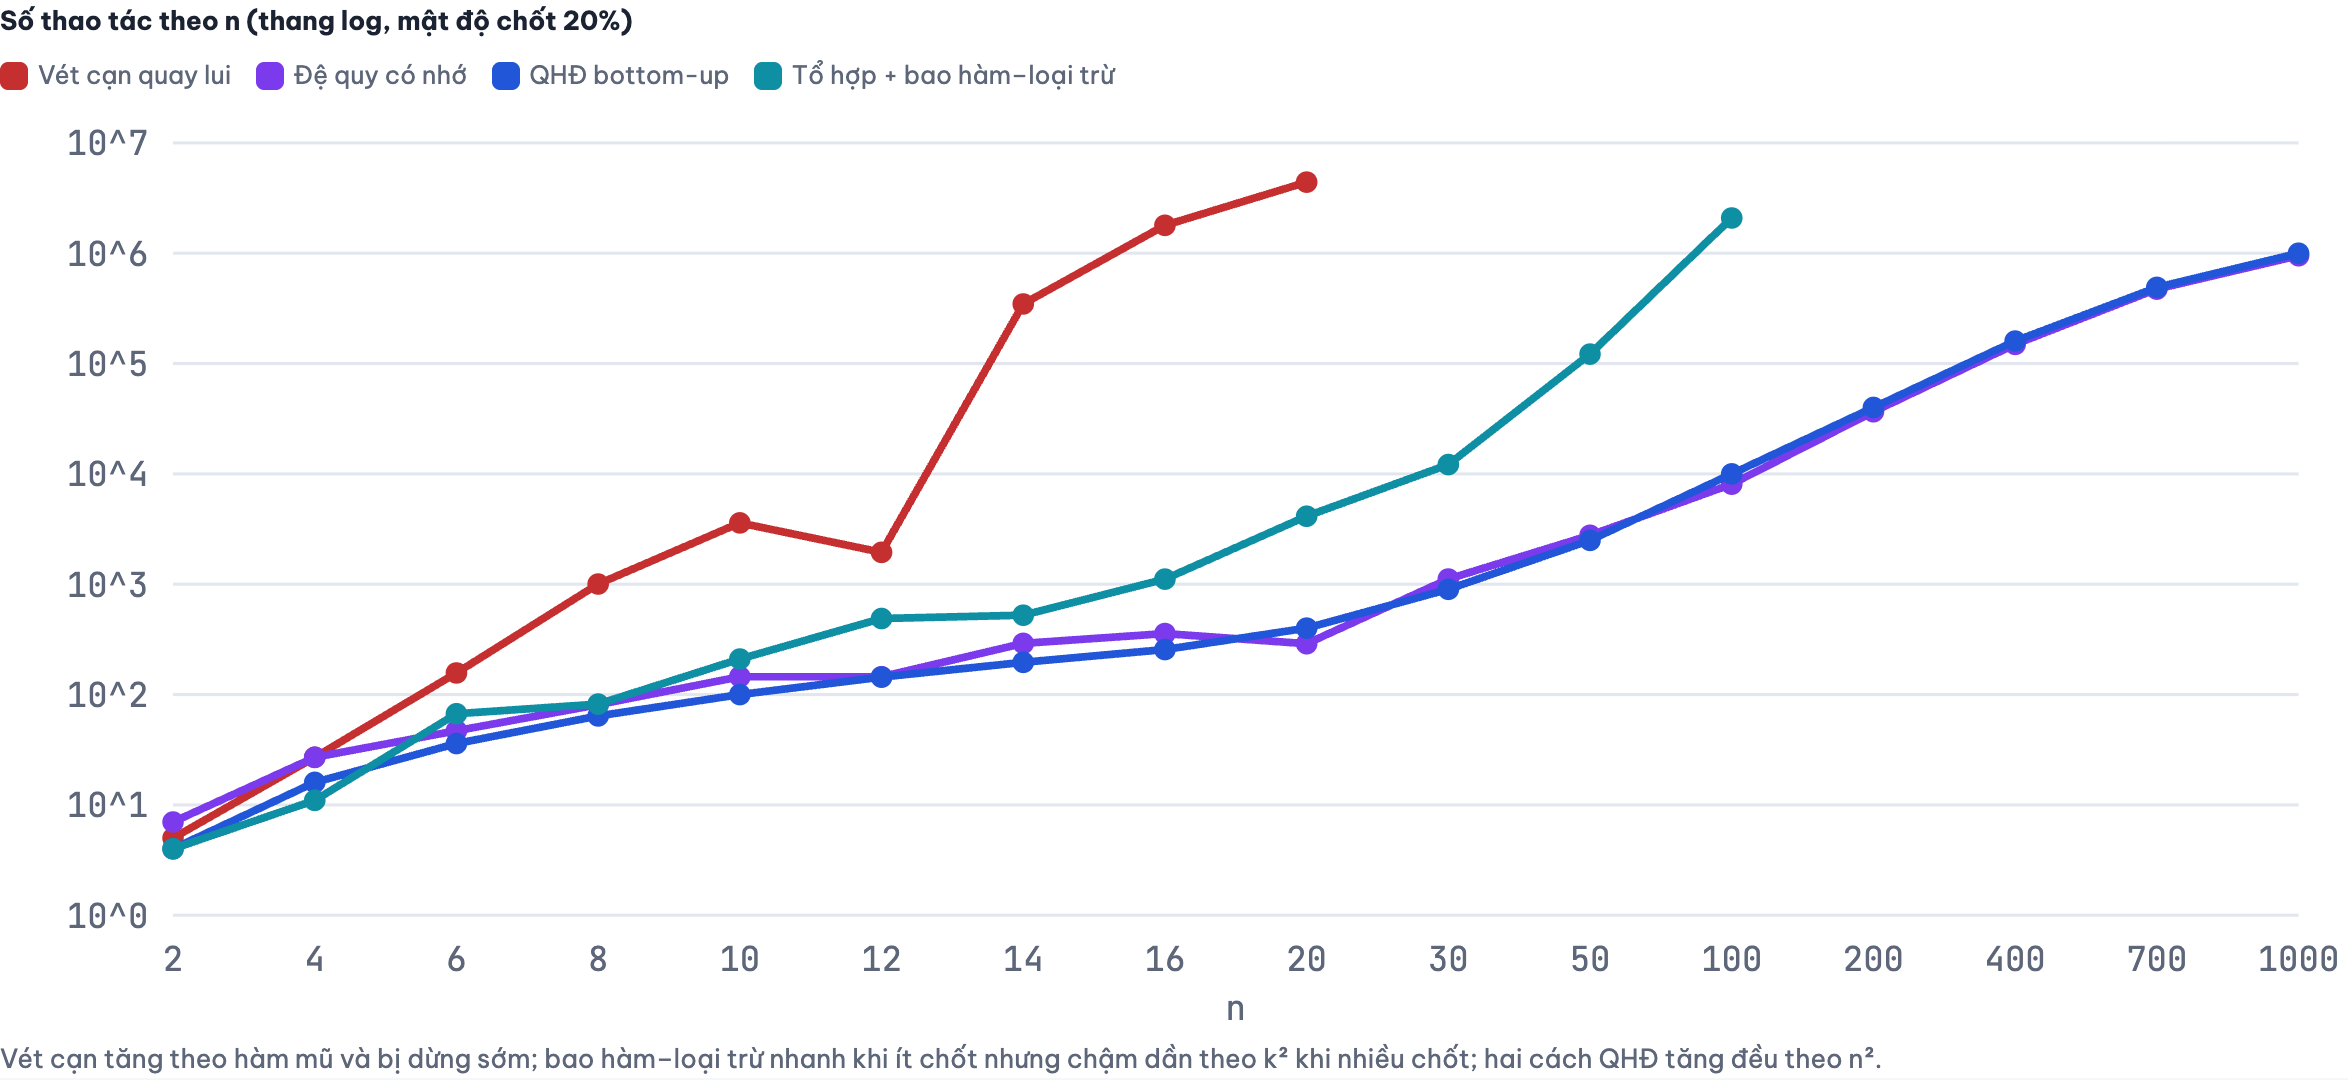
\includegraphics[width=0.49\linewidth]{img/bench20.png}
\caption{Khối ``So sánh 4 cách giải'' trên demo. Trái: bảng so sánh trên ví dụ $6\times6$ và benchmark mật độ 3\%. Phải: benchmark mật độ 20\% (thang log). Vét cạn tăng theo hàm mũ và bị dừng sau $n=20$; bao hàm--loại trừ tăng theo $k^2$; hai cách QHĐ trùng nhau theo $n^2$.}
\end{figure}

\section{Tính trực quan và khả năng minh họa}
\begin{itemize}
  \item Cả 4 cách giải đều có chế độ chạy từng bước: tiến/lùi, chạy/dừng, chỉnh tốc độ, phím tắt. Mỗi bước có hình trên lưới, câu giải thích, công thức với số cụ thể, dòng mã giả đang chạy, và bộ đếm (lời gọi, lần dùng lại bảng nhớ, độ sâu, số đường tìm được).
  \item Có kết quả ``số đường thật'' (số nguyên lớn) bên cạnh đáp án mod để người học thấy vì sao phải lấy dư; có chức năng vẽ một đường an toàn và làm mờ ô vô dụng.
  \item Chức năng tương tác: nhập tay, 4 ví dụ mẫu, sinh ngẫu nhiên, bấm vào ô để thêm/bỏ chốt, mở/tải file \texttt{.inp}, song ngữ, sáng/tối, dùng được trên điện thoại.
\end{itemize}
\begin{figure}[H]\centering
\begin{minipage}{0.48\linewidth}\centering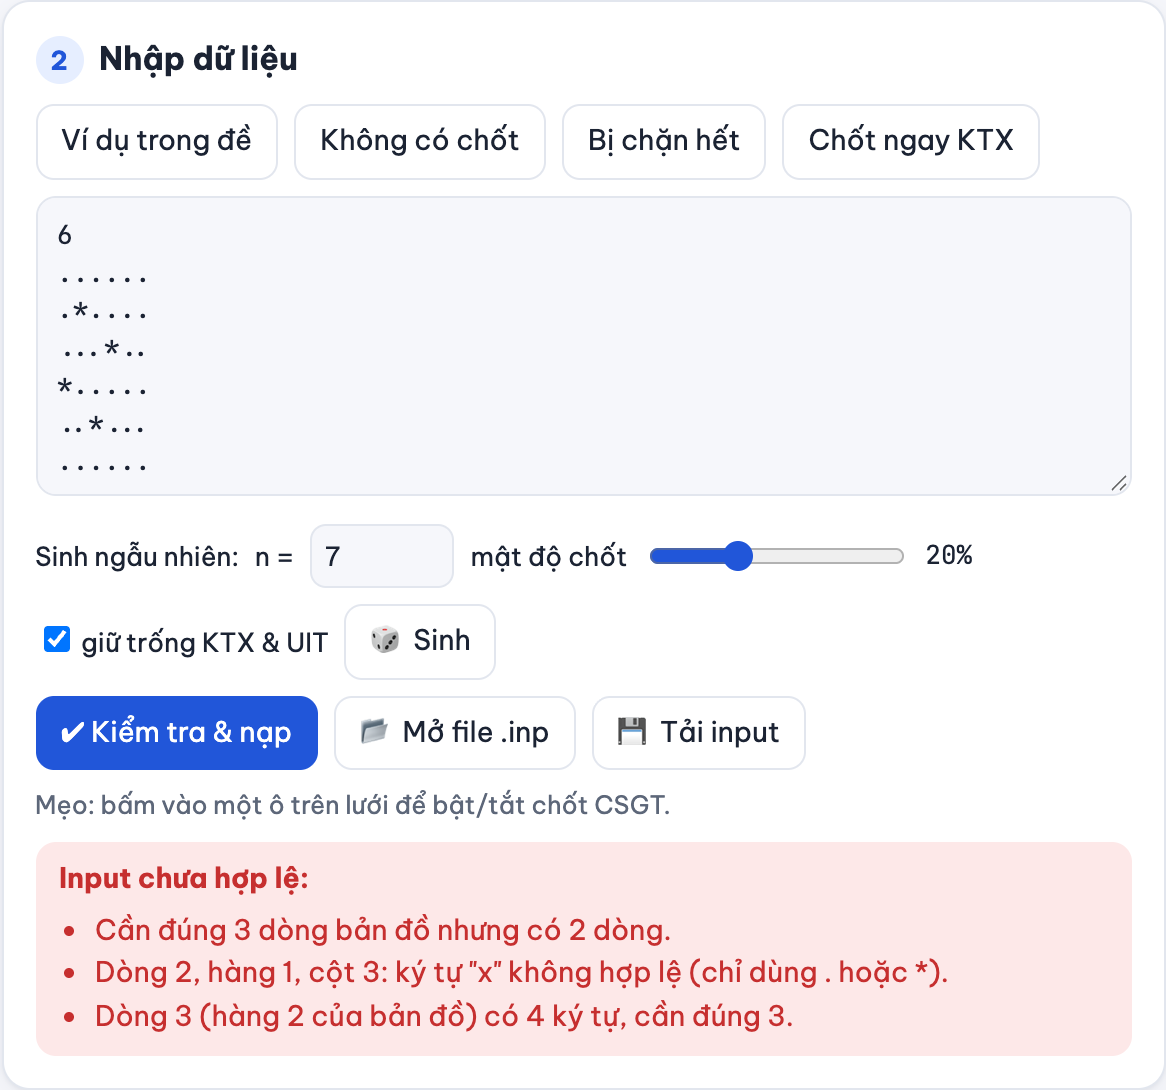
\includegraphics[width=\linewidth]{img/validate.png}\end{minipage}\hfill
\begin{minipage}{0.48\linewidth}\centering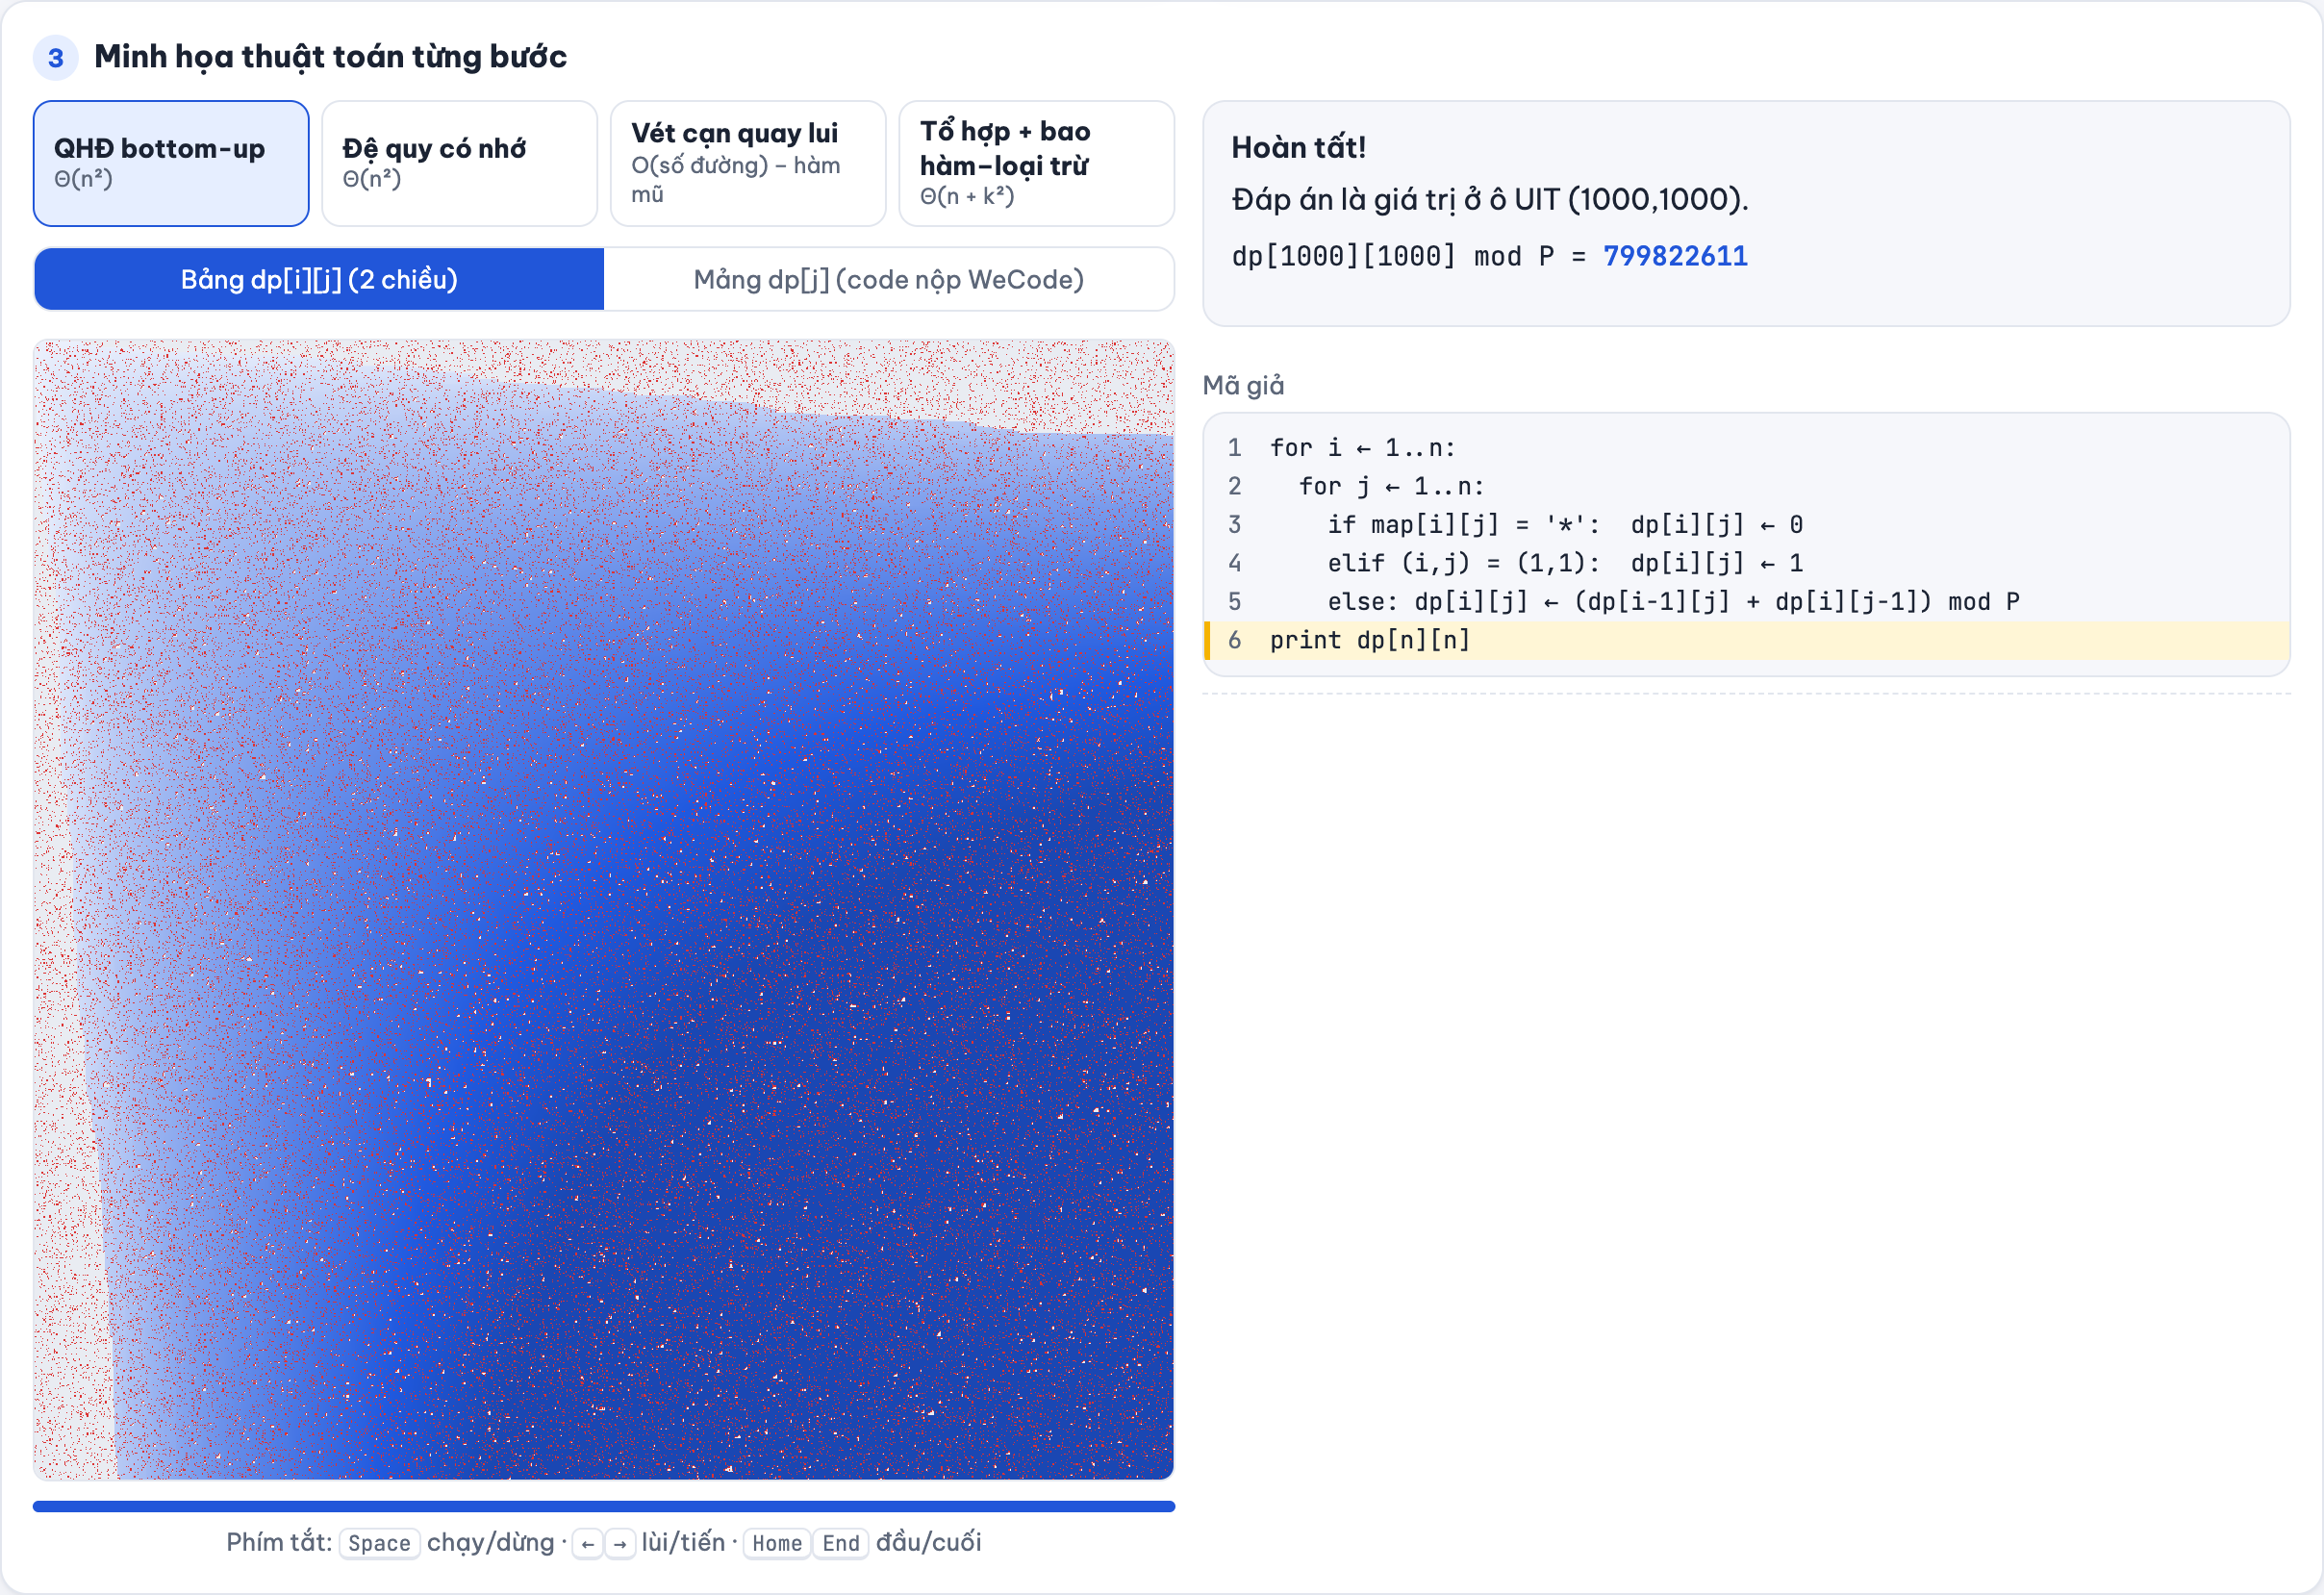
\includegraphics[width=\linewidth]{img/big.png}\end{minipage}
\caption{Trái: báo lỗi input kèm vị trí. Phải: lưới $1000\times1000$ dạng bản đồ nhiệt.}\end{figure}

\section{Hạn chế}
\begin{itemize}
  \item Minh họa từng bước chỉ áp dụng cho lưới $\le16\times16$; vét cạn chỉ minh họa 1500 bước đầu.
  \item Bao hàm--loại trừ bị giới hạn $k\le4000$ trên demo.
  \item Bản đồ nhiệt dùng số thực nên chỉ mang tính định tính.
  \item ``Số thao tác'' của mỗi cách có đơn vị khác nhau (lời gọi, ô, cặp chốt) nên chỉ so sánh được bậc tăng trưởng, không so sánh tuyệt đối.
\end{itemize}
\section{Hướng phát triển}
\begin{itemize}
  \item Biến thể: lưới chữ nhật $m\times n$, cho đi chéo, ``được phép bị thổi tối đa $t$ lần'' (QHĐ 3 chiều $dp[i][j][t]$).
  \item Tìm đường an toàn có chi phí nhỏ nhất (mỗi ô có trọng số), hoặc liệt kê đường theo thứ tự từ điển (kết hợp QHĐ đếm + truy vết).
  \item Tối ưu song song hóa theo đường chéo phụ (các ô trên cùng đường chéo độc lập nhau).
\end{itemize}

% =====================================================
\begin{thebibliography}{9}
\bibitem{levitin} A. Levitin, \emph{Introduction to the Design and Analysis of Algorithms}, 3rd ed., Addison Wesley, 2011 -- Chương 8 (Dynamic Programming), Chương 12 (Backtracking).
\bibitem{clrs} T. H. Cormen, C. E. Leiserson, R. L. Rivest, C. Stein, \emph{Introduction to Algorithms}, 3rd ed., MIT Press -- Chương 15 (Dynamic Programming).
\bibitem{cses} CSES Problem Set, ``Grid Paths'' (Dynamic Programming), \url{https://cses.fi/problemset/task/1638}.
\bibitem{cf559c} Codeforces Round \#313, Problem 559C ``Gerald and Giant Chess'', \url{https://codeforces.com/problemset/problem/559/C}.
\bibitem{slide} Huỳnh Thị Thanh Thương, slide bài giảng CS112 (Quay lui, Quy hoạch động, Kỹ thuật đếm), UIT, 2026.
\end{thebibliography}

% =====================================================
\appendix
\chapter{Lời giải nộp WeCode (Python, tự viết, Accepted)}
\lstinputlisting[language=Python]{../1_SourceCode/solution/safe_path.py}

\chapter{Cấu trúc thư mục nộp}
\begin{lstlisting}[numbers=none]
DoAn_DuongDiAnToan/
  1_SourceCode/
    app/index.html, app/core.js   demo web + 4 thuat toan
    solution/safe_path.py         loi giai nop WeCode
    tools/                        script quay video, chup anh
  2_VideoDemo/demo.mp4            video demo khong loi (~3 phut 20 giay)
  3_Testcase/
    01_thong_thuong/ ... 06_khong_hop_le/   103 test (.inp/.out)
    gen_tests.py, run_tests.py, run_js.js, manifest.json
    ket_qua/                      ket qua chay test (csv, md)
  4_Report/report.tex, report.pdf, tables.tex, gen_tables.js, img/
\end{lstlisting}
\end{document}
